\documentclass[a4paper]{ifacconf}

\usepackage{graphicx,amsmath,amssymb,booktabs,siunitx,multirow,url,placeins}
\usepackage[table]{xcolor}
\usepackage{soul}
\usepackage[round]{natbib}

% Destaque de revisão: todo o texto alterado nesta revisão é marcado em amarelo.
\sethlcolor{yellow}
\soulregister\cite7
\soulregister\citep7
\soulregister\citet7
\soulregister\ref7
\newcommand{\rev}[1]{\hl{#1}}

\usepackage[english,brazil]{babel}

\usepackage[T1]{fontenc}
\usepackage[utf8]{inputenc}
\usepackage{ae}
\usepackage{icomma}

\graphicspath{{./figuras/}}

\makeatletter
\def\@keywordheading{{\itshape Palavras-chave: }}
\makeatother

\begin{document}

\begin{frontmatter}

\title{Predição da Qualidade da Água: Inferência Neuromórfica Multimodal Offline com Consciência Energética na Borda\thanksref{footnoteinfo}}

\thanks[footnoteinfo]{Os autores agradecem o apoio financeiro do Instituto de Pesquisas Eldorado, da Motorola Mobility Com\'ercio de Produtos Eletr\^onicos Ltda, da Flextronics da Amaz\^onia Ltda e do projeto de PD\&I ``Mob4Ai -- Advanced Artificial Intelligence for Neuromorphic Mobile Systems'' (Conv\^enio n\textordmasculine~008/2024, nos termos do Decreto n\textordmasculine~10.521/2020 e da Lei Federal n\textordmasculine~8.387/1991).}

\author[UFAM,ELD,PPGCTS]{Felipe de Vasconcelos Assun\c{c}\~ao}
\author[UFAM,PPGCTS]{Alfredo Paulo Oliveira Barros}
\author[UFAM]{Reyner Carlos Silva Alegria}
\author[IND]{Elton dos Santos Ara\'ujo}
\author[ELD]{D\'ebora Romano Raimundo}
\author[UFAM]{Alex Martins Ramos}
\author[UFAM]{Vicente Ferreira de Lucena Junior}
\author[UFAM,PPGCTS]{Vandermi Jo\~ao da Silva}

\address[UFAM]{Universidade Federal do Amazonas (UFAM), Instituto de Ci\^encias Exatas e Tecnologia (ICET), Itacoatiara, Brasil (e-mail: \{felipe.assuncao, alfredo.barros, reyner.alegria, alexmartins, vicente, vandermi\}@ufam.edu.br).}
\address[IND]{Pesquisador Independente, Brasil (e-mail: elton\_araujo\_@hotmail.com).}
\address[ELD]{Instituto de Pesquisas Eldorado, Brasil (e-mail: debora.raimundo@eldorado.org.br, felipe.assuncao@eldorado.org.br).}
\address[PPGCTS]{Programa de P\'os-Gradua\c{c}\~ao em Ci\^encia, Tecnologia e Sa\'ude (PPGCTS), Brasil.}

\renewcommand{\abstractname}{{\bf Resumo:~}}
\begin{abstract}
Este trabalho apresenta um pipeline neuromórfico centrado em Edge AI para a predição multimodal da qualidade da água em um cenário remoto da Amazônia. O objetivo central é a implantação totalmente offline em hardware restrito, evitando a dependência de nuvem sob conectividade limitada e orçamentos de energia reduzidos. Uma rede neural pulsada (SNN) é utilizada para predizer conjuntamente pH, oxigênio dissolvido e turbidez a partir de entradas físico-químicas georreferenciadas \rev{coletadas em uma campanha de campo com 60 amostras georreferenciadas}. Para melhorar a estabilidade em condições de poucos dados, aplicamos aumento de dados gaussiano controlado \rev{(expandindo o suporte de treinamento em dez vezes, para 600 amostras)} e otimizamos o modelo por meio de busca em grade sistemática sobre passos temporais, taxa de aprendizado, limiar, decaimento e tamanho da camada oculta. A SNN multimodal resultante é avaliada com protocolos de múltiplas sementes \rev{reportados com intervalos de confiança de 95\% e testes de significância não paramétricos (Wilcoxon pareado exato e Friedman)} e, em seguida, implantada em plataformas de borda heterogêneas (ESP32, Raspberry Pi e dispositivos Android). Reportamos vazão, latência e energia incremental por inferência usando medições em repouso/carga, incluindo telemetria baseada em INA219 quando aplicável. Os resultados mostram que, embora Random Forest e LSTM possam alcançar menor erro macro médio, a SNN permanece competitiva e operacionalmente robusta para cenários de borda, viabilizando inferência offline prática em hardware das classes microcontrolador, SBC e smartphone. De forma geral, o estudo demonstra que a Edge AI neuromórfica é uma estratégia viável para o monitoramento ambiental autônomo em regiões com restrições de conectividade e energia.
\end{abstract}

\begin{keyword}
Redes Neurais Pulsadas; Edge AI; Avaliação Energética; Predição da Qualidade da Água; Modelagem Multimodal; Inferência Offline.
\end{keyword}

\end{frontmatter}

\section{Introdução}

O monitoramento da qualidade da água em áreas remotas da Amazônia é limitado pela infraestrutura esparsa, pelo alto custo logístico das campanhas de campo e pela conectividade de rede intermitente. A implantação de Edge AI é a motivação central deste trabalho: a inferência local, totalmente offline, é necessária para manter o monitoramento funcional sob comunicações instáveis e orçamentos de energia limitados. Nesse contexto, a dependência contínua de inferência em nuvem é operacionalmente frágil e energeticamente cara, especialmente em implantações alimentadas por bateria e campanhas de longa duração. Ao mesmo tempo, variáveis de qualidade da água como pH, oxigênio dissolvido (OD) e turbidez são altamente relevantes para a triagem ambiental e a mitigação de riscos à saúde pública.

Pipelines convencionais de aprendizado de máquina podem oferecer forte desempenho preditivo, mas muitos são projetados para execução centrada em servidores e não tratam diretamente as restrições energéticas na borda. Modelos neuromórficos baseados em redes neurais pulsadas (SNNs, do inglês \textit{spiking neural networks}) oferecem uma alternativa orientada a eventos, compatível com sistemas embarcados de baixo consumo; contudo, evidências práticas em fluxos reais de sensoriamento ambiental ainda são limitadas, particularmente quando se combinam predição multimodal e avaliação energética em nível de plataforma.

Este artigo propõe e avalia um pipeline SNN multimodal offline para predição da qualidade da água em um cenário de campo amazônico, incluindo implantação de ponta a ponta e análise energética multiplataforma. O estudo integra processamento de dados, treinamento de modelos, interpretação geoespacial e inferência embarcada em hardware heterogêneo (ESP32, Raspberry Pi e dispositivos Android).

As principais contribuições deste trabalho são \rev{quatro}: (i) o desenvolvimento de um pipeline de predição da qualidade da água baseado em SNN multimodal, projetado para implantação offline na borda; (ii) a criação de um conjunto de dados georreferenciado aumentado, derivado de medições de campo no Lago do Serpa; (iii) uma avaliação comparativa de latência--energia em plataformas heterogêneas, incluindo ESP32, Raspberry Pi e dispositivos Android\rev{; e (iv) um protocolo de avaliação estatisticamente fundamentado para regressão ambiental com poucos dados, combinando avaliação com sementes repetidas, intervalos de confiança e testes de significância não paramétricos. Para além da avaliação energética, a contribuição científica reside em demonstrar, de ponta a ponta, que a regressão neuromórfica multimodal de alvos físico-químicos de qualidade da água é viável desde a aquisição em campo até a inferência totalmente offline em três classes distintas de hardware de borda --- uma combinação ainda não reportada para o monitoramento de água doce na região amazônica.}

\section{Trabalhos Relacionados}

\subsection{Predição da Qualidade da Água}
A predição orientada a dados de indicadores de qualidade da água tem sido amplamente explorada com RNAs, modelos baseados em árvores e arquiteturas recorrentes. Revisões e estudos recentes reportam o uso consistente de variáveis físico-químicas e de contexto geoespacial para prever pH, OD, turbidez e indicadores compostos \cite{yan2024,ahmed2019,aladhaileh2021,pan2025}. Abordagens baseadas em LSTM são comuns onde os registros temporais são densos \cite{liu2019,pyo2023,qi2020}, enquanto métodos híbridos e de comitês melhoram a robustez sob comportamento não linear e regimes de amostragem limitados \cite{wu2022,chadalavada2025,kalaivanan2022,palani2008}.

Além da escolha do modelo, uma distinção importante na literatura é o objetivo operacional: máxima acurácia preditiva em infraestrutura centralizada versus robustez sob sensoriamento ruidoso, amostragem esparsa e restrições de campo, uma distinção crítica para águas interiores, onde o comportamento do modelo é afetado pela heterogeneidade local, pela sazonalidade e pela incerteza de medição \cite{yan2024,lowe2022,rahu2023}.

\subsection{Edge AI e Avaliação Energética}
Em implantações de IoT ambiental, o custo de inferência deve ser avaliado em conjunto com a qualidade preditiva. Trabalhos anteriores destacam a relevância do benchmarking em nível de plataforma e do projeto de modelos ciente do hardware \cite{rosero2020,zulkifli2022,lamrini2024,elshafeiy2023}. Estudos recentes de IA neuromórfica e energeticamente eficiente indicam que modelos orientados a eventos podem ser atraentes para cenários restritos, mas as evidências de implantação em hardware de borda heterogêneo ainda estão em desenvolvimento \cite{aral2024,azadi2025,huijbregts2024,aribe2025future}. Essa lacuna motiva o presente trabalho: uma comparação unificada da qualidade de inferência multimodal offline e do comportamento de energia por inferência em múltiplas plataformas práticas.

A maioria dos estudos anteriores reporta métricas algorítmicas ou métricas de hardware isoladamente. Em contraste, a implantação em campo requer uma visão acoplada de latência, vazão e energia incremental sob transições realistas de repouso/carga. Consequentemente, o benchmarking multiplataforma deve ser interpretado como um resultado de sistemas, e não apenas como um resultado de modelo.

\rev{Posicionar este trabalho frente a estudos recentes de monitoramento ambiental neuromórfico esclarece sua novidade. \citet{aral2024} discutem a promessa da Edge AI neuromórfica para monitoramento rural em nível conceitual, sem implantação em campo; \citet{azadi2025} demonstram inferência neuromórfica embarcada para IoT industrial, mas não para regressão de qualidade da água; \citet{huijbregts2024} tratam da eficiência de SNNs em nível de circuito; e \citet{alshareeda2025} implantam monitoramento de água baseado em ESP32 sem modelos neuromórficos. Até onde sabemos, nenhum estudo anterior combina regressão SNN multimodal de alvos físico-químicos, dados de campo de um lago amazônico e energia por inferência medida em hardware das classes microcontrolador, SBC e smartphone em um único pipeline offline, que é a lacuna aqui abordada.}

\section{Descrição do Conjunto de Dados}

A campanha de campo foi conduzida em um ambiente de água doce na região amazônica (Itacoatiara, AM, Brasil), com pontos de amostragem georreferenciados distribuídos para capturar gradientes espaciais locais. O conjunto de dados inclui a posição em UTM 21S e variáveis físico-químicas usadas como entradas e saídas do modelo, e está publicamente disponível no Mendeley Data \cite{assuncao2026dataset}. A cobertura espacial da campanha é mostrada na Fig.~\ref{fig:dataset_map}, e as estatísticas descritivas dos alvos de predição são reportadas na Tabela~\ref{tab:dataset_stats}.

A coleta de dados seguiu um desenho espacialmente distribuído para representar diferentes microzonas do lago, em vez de amostrar repetidamente uma única coordenada, apoiando a interpretação espacial e o suporte à decisão local (mapas de interpolação e índices compostos de triagem). As medições foram consolidadas em uma estrutura tabular adequada à inferência orientada à borda e ao treinamento reprodutível.

\subsection{Variáveis e Aquisição}
Os atributos de entrada foram $x$, $y$, temperatura (TEMP), cor aparente em escala âmbar (COR\_A) e índice visual de cor (COR\_V). As variáveis-alvo foram pH, oxigênio dissolvido (OD) e turbidez (TURB). \rev{O conjunto de dados original de campo compreende 60 amostras georreferenciadas.} O desenho amostral priorizou a representatividade espacial em detrimento da repetição temporal densa, de forma consistente com o objetivo de gerar superfícies espaciais interpretáveis.

\rev{A Tabela~\ref{tab:corr_analysis} reporta a correlação de Pearson entre cada atributo de entrada e cada alvo no conjunto original de 60 amostras. As coordenadas espaciais e os índices de cor estão fortemente associados ao pH (\mbox{$r=-0,85$} para $y$; \mbox{$r=-0,79$} para COR\_A) e à turbidez (\mbox{$r=0,69$} e \mbox{$r=0,68$}, respectivamente), indicando gradientes espaciais e ópticos exploráveis. Em contraste, o OD é fracamente correlacionado com todas as entradas disponíveis (\mbox{$|r| \leq 0,24$}), o que antecipa a maior dificuldade de predição desse alvo com o conjunto de atributos atual.}

\begin{table}[t]
\caption{\rev{Correlação de Pearson entre atributos de entrada e alvos (conjunto original, $n=60$).}}
\label{tab:corr_analysis}
\centering
\footnotesize
\setlength{\tabcolsep}{6pt}
\rowcolors{2}{yellow!30}{yellow!30}
\begin{tabular}{lccc}
\toprule
Atributo & pH & OD & TURB \\
\midrule
$x$ & $0.75$ & $-0.23$ & $-0.67$ \\
$y$ & $-0.85$ & $0.18$ & $0.69$ \\
TEMP & $-0.56$ & $0.24$ & $0.33$ \\
COR\_A & $-0.79$ & $0.05$ & $0.68$ \\
COR\_V & $-0.46$ & $0.08$ & $0.50$ \\
\bottomrule
\end{tabular}
\end{table}

\begin{figure}[t]
\centering
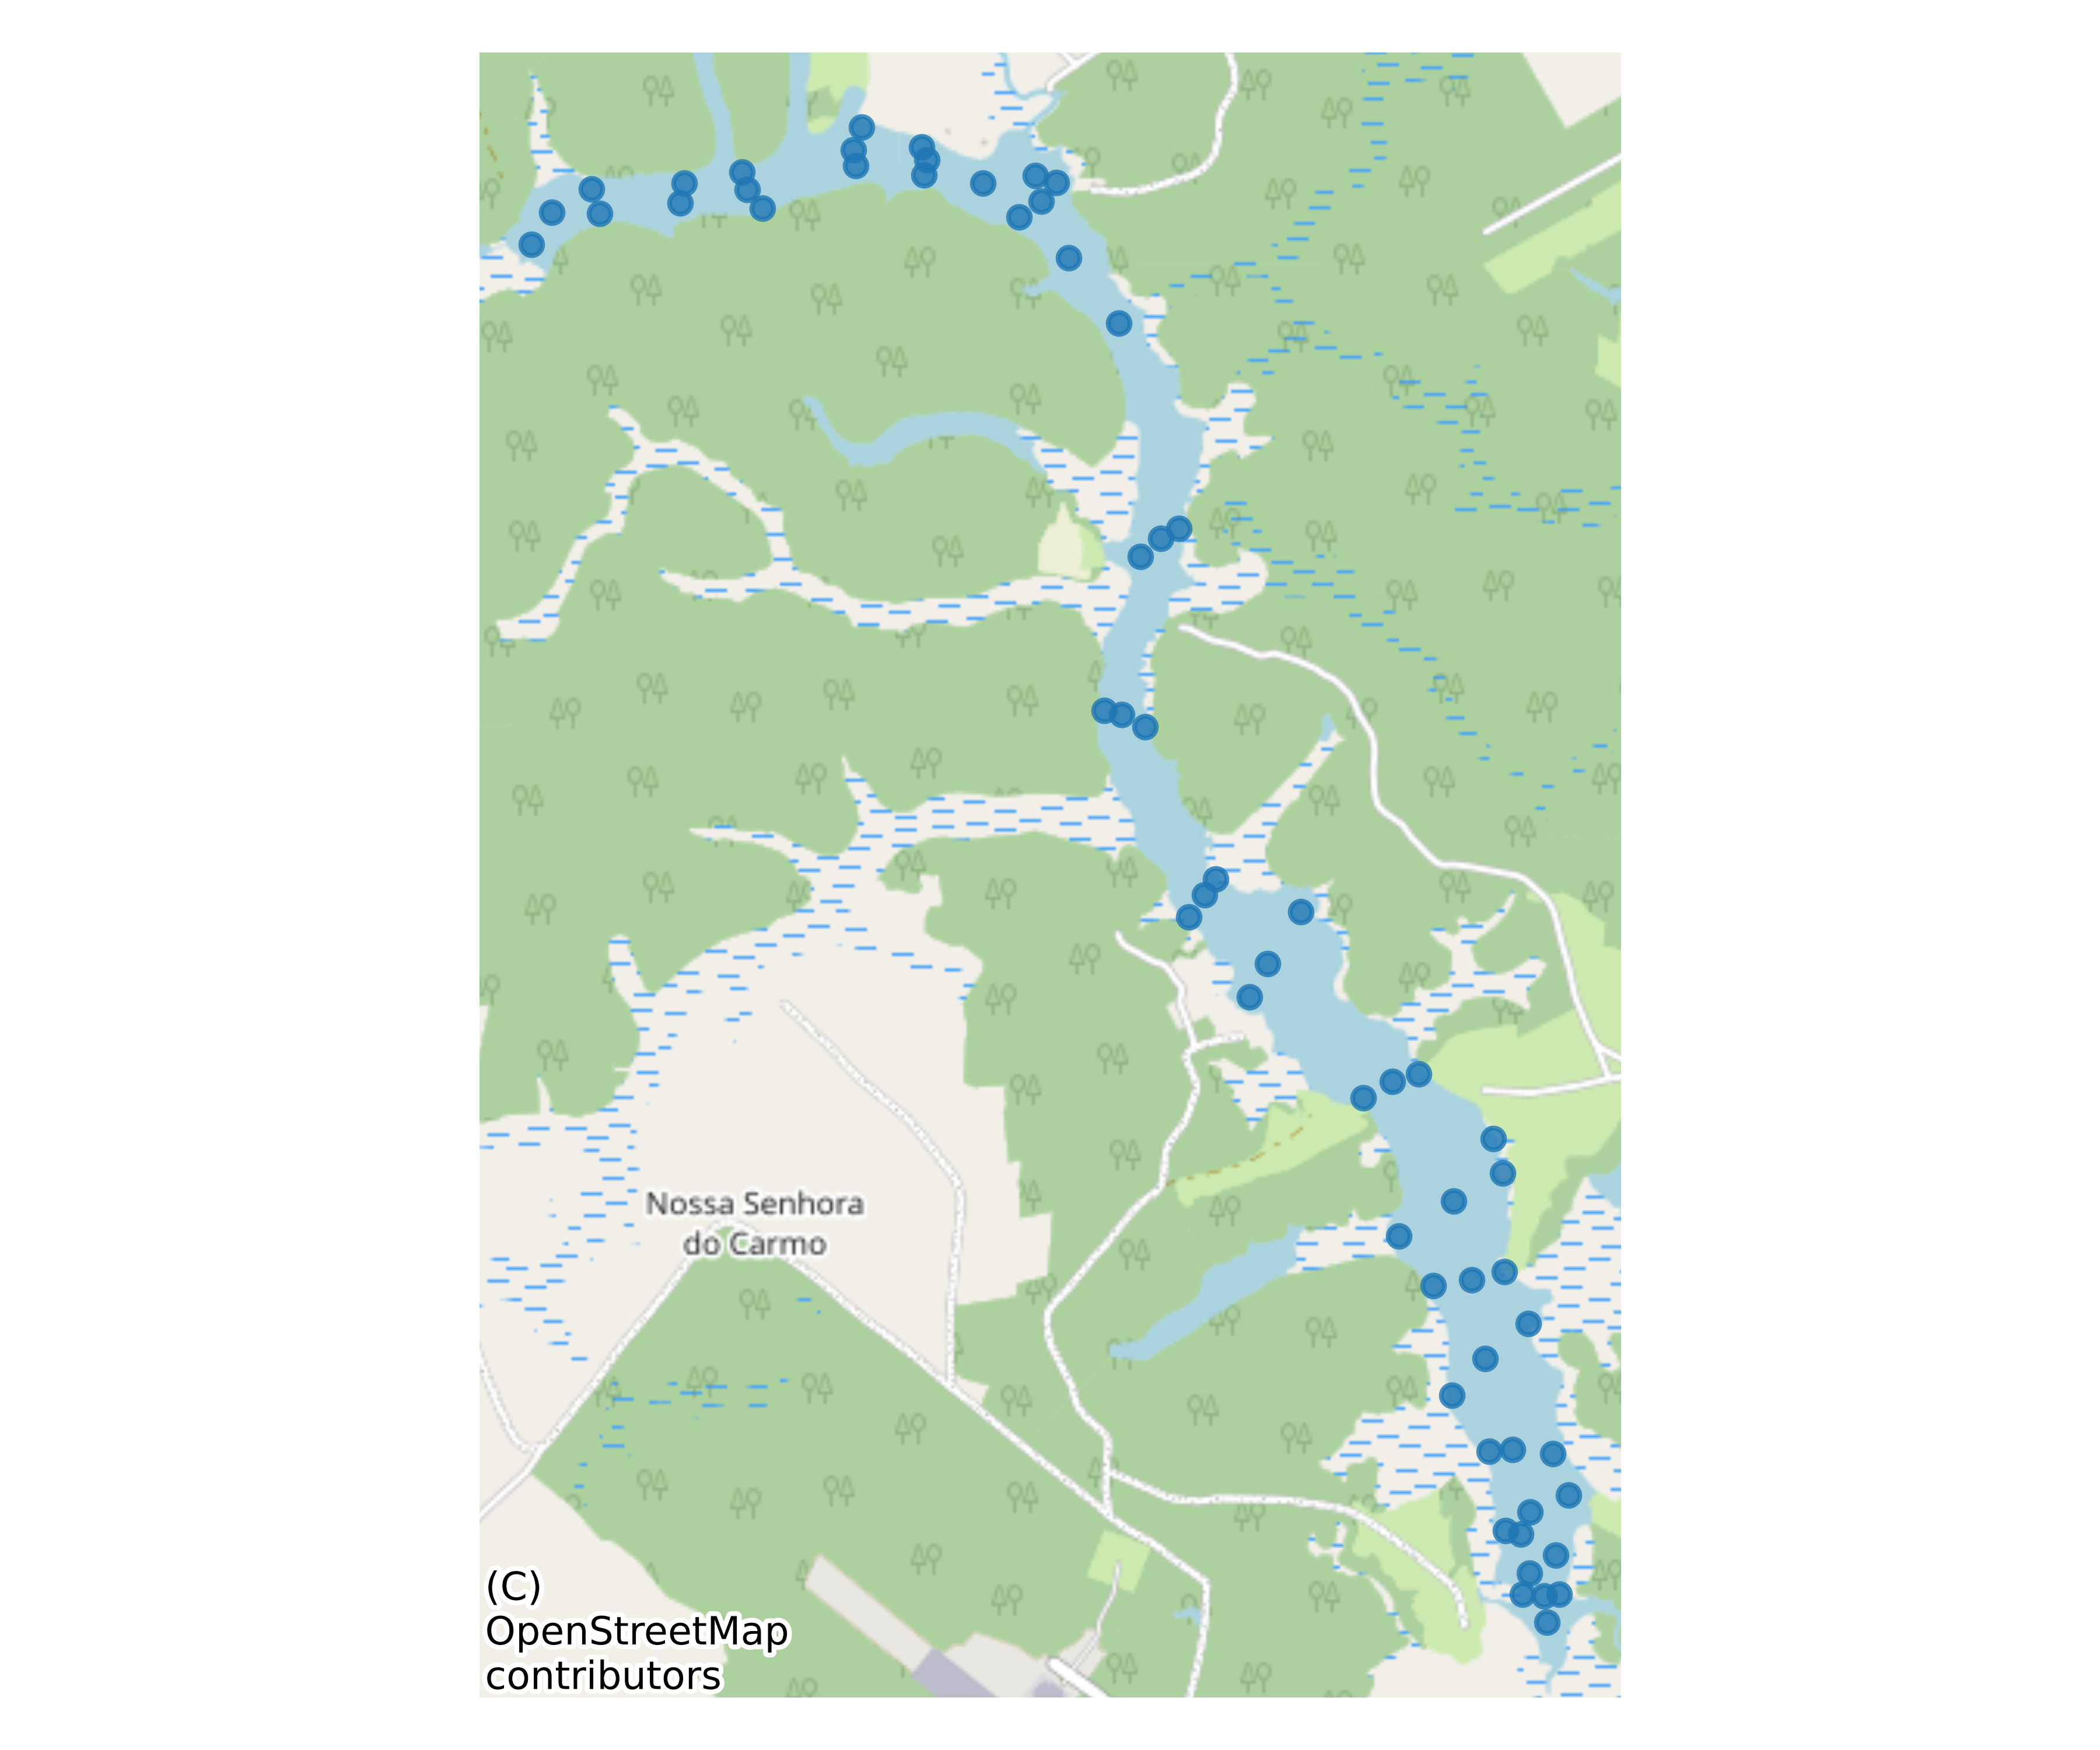
\includegraphics[width=0.64\linewidth]{map_points_osm_21S.png}
\caption{Localizações de amostragem sobre mapa-base OpenStreetMap (UTM 21S).}
\label{fig:dataset_map}
\end{figure}

\begin{table}[t]
\caption{Estatísticas descritivas dos alvos no conjunto de dados original de campo.}
\label{tab:dataset_stats}
\centering
\begin{tabular}{lcccc}
\toprule
Variável & Média & Desvio & Mín & Máx \\
\midrule
pH & 5.73 & 0.31 & 5.15 & 6.50 \\
OD (mg/L) & 1.86 & 0.32 & 1.26 & 2.52 \\
Turbidez (NTU) & 2.77 & 1.37 & 0.06 & 6.18 \\
\bottomrule
\end{tabular}
\end{table}

\subsection{Aumento de Dados}
Como o conjunto de dados original é pequeno \rev{($n=60$)}, aplicou-se aumento sintético com fator $\times 10$ usando perturbação gaussiana leve (\mbox{$\sigma=0,01$}) no espaço normalizado\rev{, resultando em 600 amostras de suporte ao treinamento}. Essa estratégia foi usada para estabilizar o treinamento e reduzir a sensibilidade à partição, preservando as distribuições marginais e a plausibilidade física. O conjunto aumentado é usado apenas como suporte ao treinamento e não representa medições de campo adicionais. \rev{A perturbação gaussiana foi adotada por sua transparência e baixo risco de distorção neste regime; estratégias alternativas de aumento para pequenos conjuntos tabulares, como interpolação no estilo SMOTE para regressão, mixup e abordagens generativas (p.~ex., síntese baseada em cópulas ou GANs), são candidatas naturais a uma comparação sistemática em trabalhos futuros.}

Para minimizar o risco de distorção, o aumento foi restrito a perturbações de baixa amplitude e avaliado com verificações distribucionais e análise de ablação: o objetivo foi aumentar a densidade local em torno das amostras observadas e melhorar a estabilidade da otimização entre partições aleatórias, e não criar dinâmicas sintéticas ausentes da campanha de campo.

Por fim, o conjunto de dados deve ser interpretado como um benchmark regional inicial, e não como uma representação hidrológica universal. A amostragem atual apoia a modelagem comparativa e a análise de implantação, enquanto a generalização externa mais ampla requer campanhas em múltiplas estações e sítios adicionais de água doce com diferentes perfis hidrodinâmicos e antrópicos. \rev{O pequeno tamanho amostral impõe limites metodológicos concretos: os valores absolutos das métricas carregam ampla incerteza, pequenas diferenças entre modelos podem não ser estáveis entre reamostragens e a amostragem de uma única estação não captura a sazonalidade hidrológica. Esses limites motivaram o protocolo conservador aqui adotado (sementes repetidas, intervalos de confiança e testes não paramétricos) e restringem o escopo das conclusões a afirmações comparativas e orientadas à implantação.}

\section{Metodologia}

\subsection{Representação Multimodal de Entrada}
Para evitar ambiguidade entre variáveis simbólicas e nomes de sensores, representamos cada observação por um vetor de atributos multimodal ordenado:
\begin{equation}
\mathbf{x} = [x, y, \text{TEMP}, \text{COR}_{A}, \text{COR}_{V}] \in \mathbb{R}^{5},
\end{equation}
e um vetor-alvo de três saídas:
\begin{equation}
\mathbf{y} = [\text{pH}, \text{OD}, \text{TURB}] \in \mathbb{R}^{3}.
\end{equation}
Os atributos de entrada são normalizados antes da codificação em pulsos. Em seguida, aplicamos codificação por taxa (\textit{rate coding}), de modo que cada escalar normalizado é convertido em um trem de pulsos ao longo de $T$ passos de tempo, com probabilidade de disparo proporcional à sua magnitude. Isso produz uma representação temporal compatível com a dinâmica LIF subsequente, preservando a estrutura multimodal da amostra original.

\subsection{Arquitetura da SNN}
O modelo segue uma SNN \textit{feed-forward} com topologia $5 \rightarrow 64 \rightarrow 3$ e uma camada oculta de neurônios \textit{leaky integrate-and-fire} (LIF), como ilustrado na Fig.~\ref{fig:proposed_arch}. A atualização da membrana é
\begin{equation}
\mathbf{u}_{t+1} = \beta\,\mathbf{u}_{t} + \mathbf{W}\mathbf{s}_{t} - \theta\,\mathbf{z}_{t},
\end{equation}
onde $\beta$ é o decaimento da membrana, $\theta$ é o limiar de disparo e $\mathbf{z}_t$ são os pulsos emitidos. A predição de saída é calculada por agregação temporal ao longo dos passos.

\begin{figure}[!htbp]
\centering
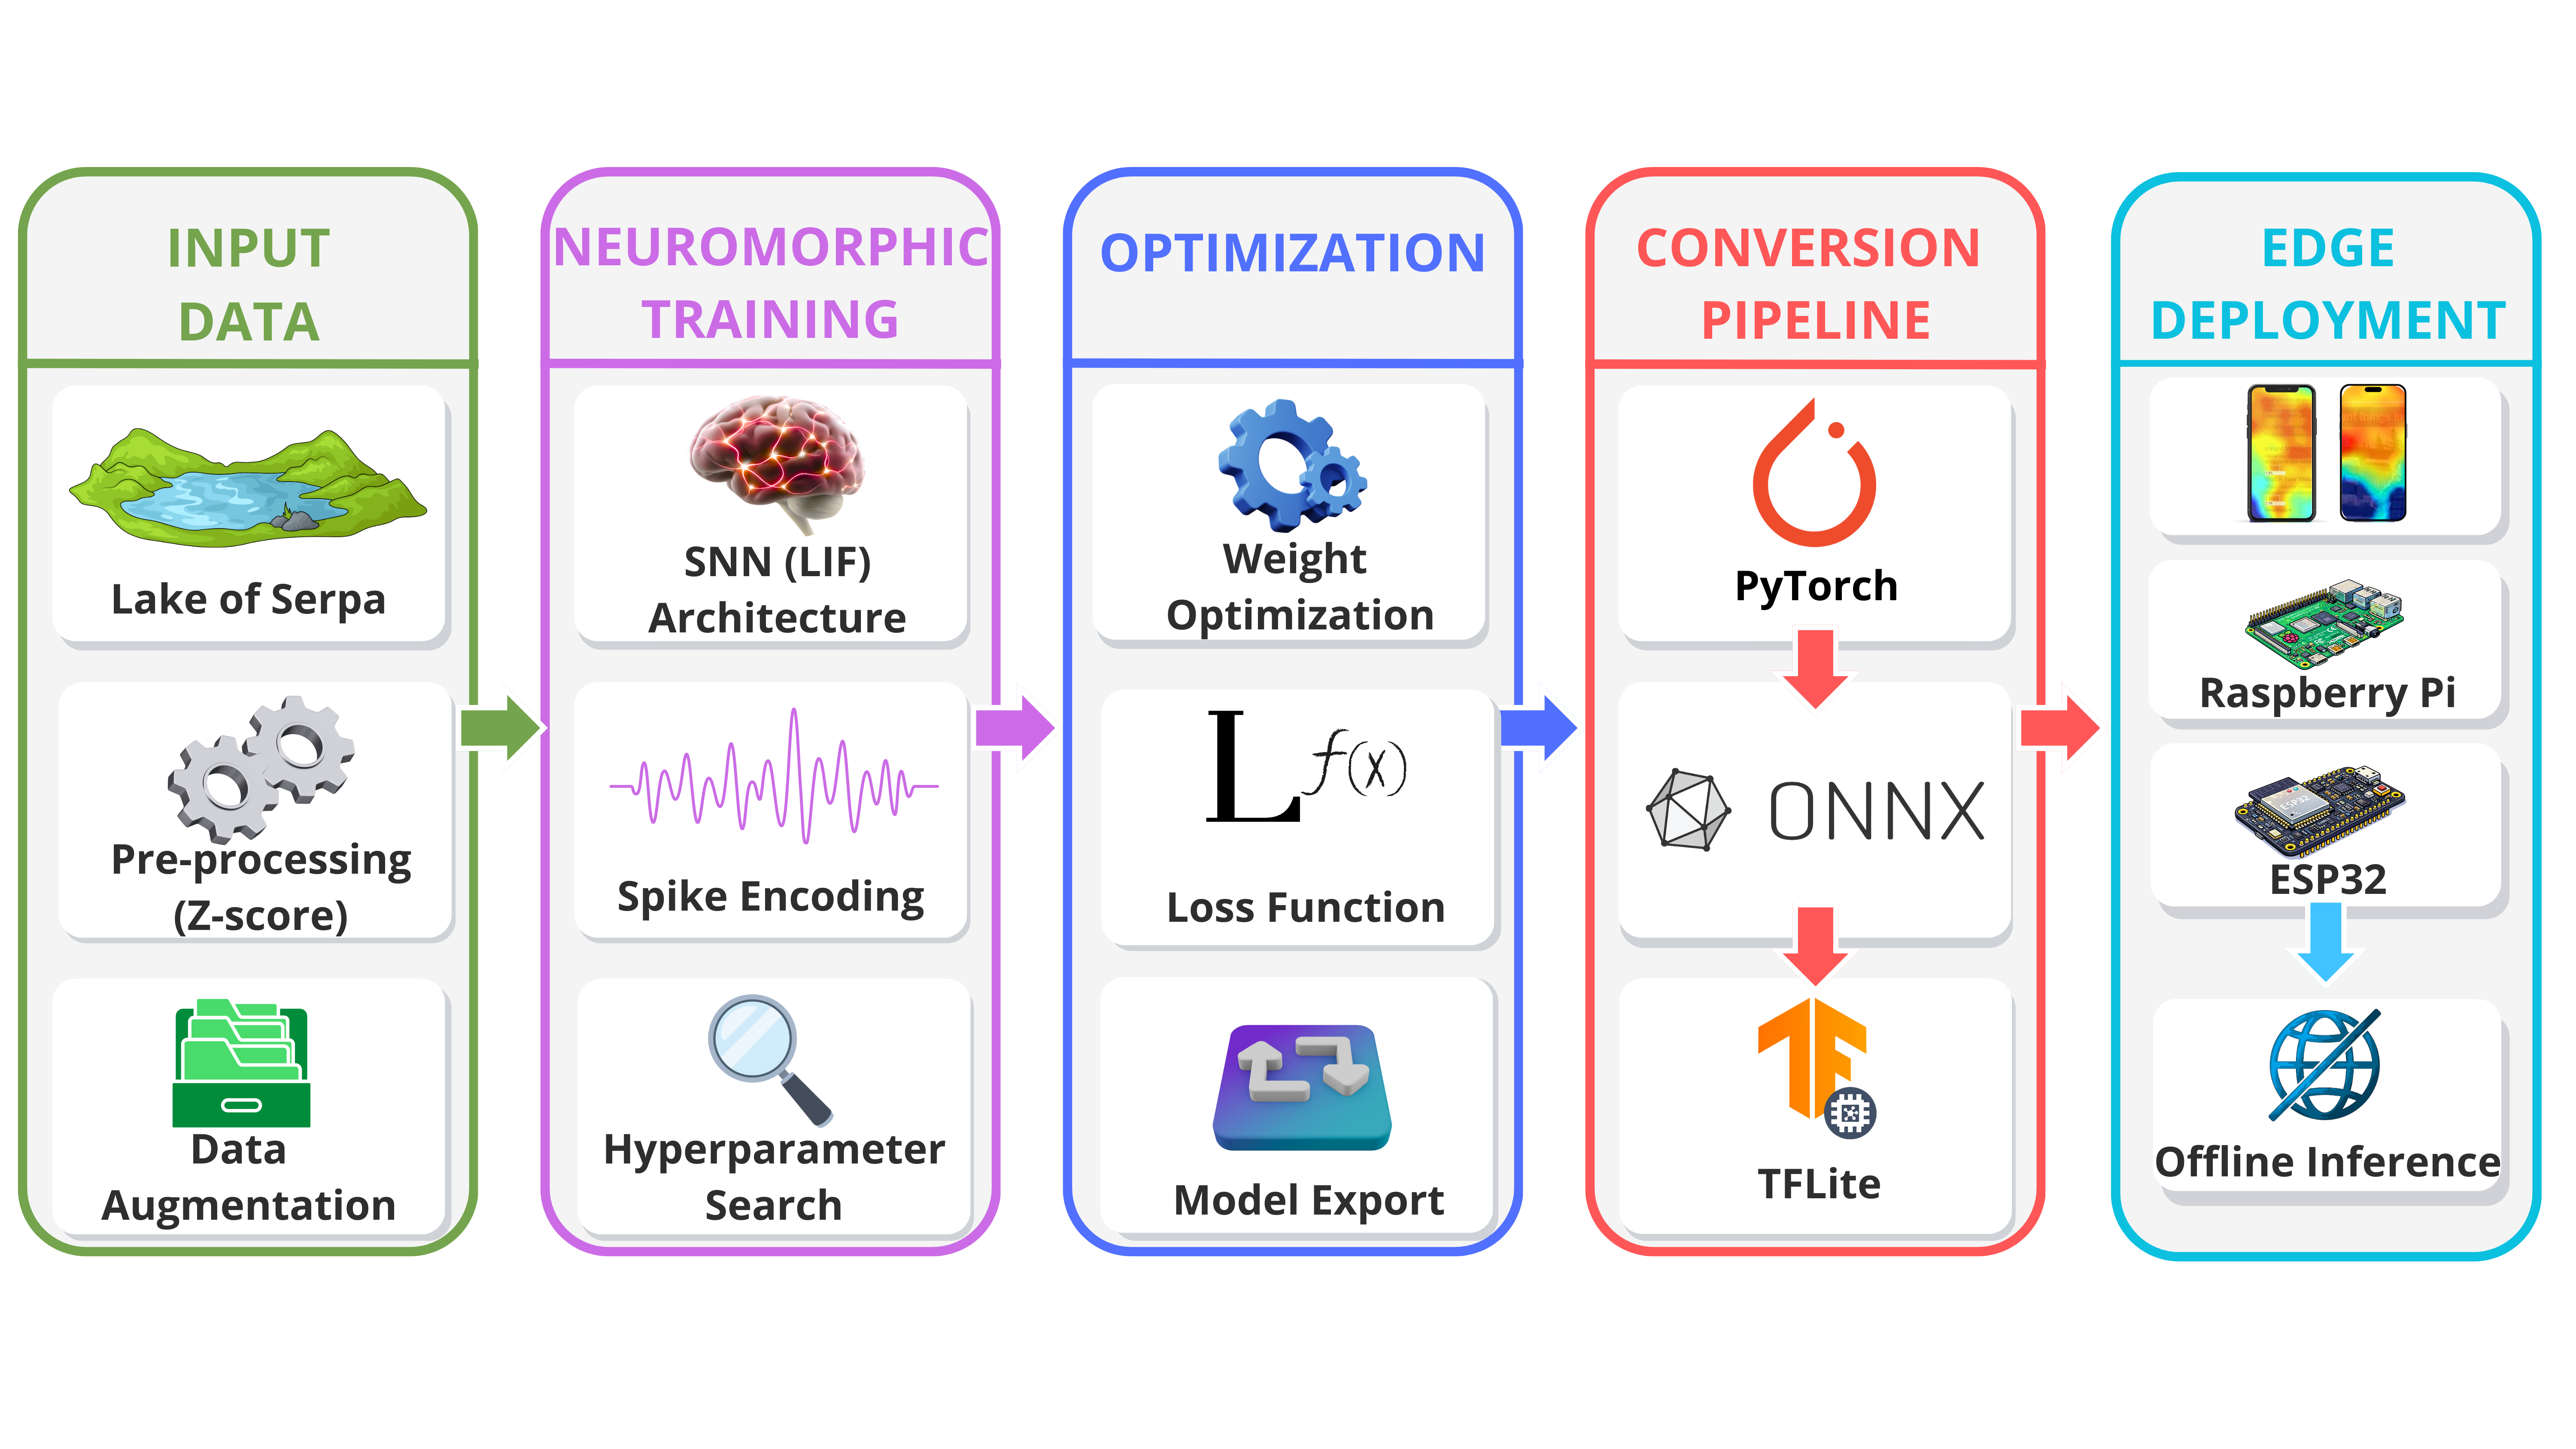
\includegraphics[width=0.58\linewidth]{Arquitetura.png}
\caption{Arquitetura SNN multimodal proposta para inferência offline na borda.}
\label{fig:proposed_arch}
\end{figure}

A Figura~\ref{fig:proposed_arch} apresenta o fluxo completo de ponta a ponta: preparação dos dados de campo (normalização e aumento controlado), treinamento neuromórfico com neurônios LIF e busca de hiperparâmetros, otimização e exportação do modelo pelo caminho de interoperabilidade PyTorch$\rightarrow$ONNX$\rightarrow$TFLite, e implantação offline na borda em Android, Raspberry Pi e ESP32.

\subsection{Protocolo de Treinamento}
O treinamento usou o otimizador Adam e perda MSE ponderada com parada antecipada. Os hiperparâmetros foram selecionados por busca em grade sobre tamanho da camada oculta, taxa de aprendizado, passos temporais $T$, limiar e fator de decaimento. \rev{O espaço de busca completo foi: tamanho da camada oculta $\in \{32, 64, 96\}$, $T \in \{10, 15, 25\}$, taxa de aprendizado \mbox{$\in \{0,0005;\, 0,001;\, 0,002\}$}, decaimento \mbox{$\beta \in \{0,90;\, 0,95\}$}, limiar \mbox{$\theta \in \{0,8;\, 1,0\}$} e ruído de aumento \mbox{$\sigma \in \{0,01;\, 0,02;\, 0,03\}$}, totalizando 324 configurações avaliadas pela perda de validação. A configuração selecionada foi: camada oculta 64, $T=15$, taxa de aprendizado \mbox{$0,002$}, \mbox{$\beta=0,95$}, \mbox{$\theta=0,8$} e \mbox{$\sigma=0,01$}.} A avaliação usou sementes aleatórias repetidas e métricas macro (MAE, RMSE e $R^2$) sobre os três alvos. \rev{As dez execuções independentes com sementes distintas implementam validação por subamostragem aleatória repetida, que aproxima o comportamento da validação cruzada neste regime de poucos dados; um protocolo k-fold completo está planejado para o conjunto de dados ampliado em campanhas futuras.}

\subsection{Sensibilidade aos Hiperparâmetros}
\rev{Os resultados da grade também fornecem uma análise de sensibilidade dos parâmetros LIF e da codificação temporal. Calculando a média marginal da perda de validação sobre as 324 configurações, a taxa de aprendizado teve o efeito mais forte (perda média de 0,826 em 0,0005 vs.~0,694 em 0,002). O limiar LIF mostrou preferência consistente por \mbox{$\theta=0,8$} em relação a \mbox{$\theta=1,0$} (0,747 vs.~0,769), enquanto o fator de decaimento teve influência menor (0,754 em \mbox{$\beta=0,90$} vs.~0,762 em \mbox{$\beta=0,95$}). O parâmetro temporal $T$ teve efeito fraco na acurácia (perda média de 0,766; 0,760 e 0,748 para \mbox{$T=10, 15, 25$}), mas o custo de inferência cresce aproximadamente de forma linear com $T$, já que cada passo adicional implica mais uma propagação direta de pulsos. Portanto, nesta tarefa, $T$ é primariamente um controle de energia--latência, e não de acurácia, e $T=15$ foi mantido como ponto de operação equilibrado.}

Como mostra a Fig.~\ref{fig:loss_curve_method}, as perdas de treinamento e validação diminuem rapidamente nas épocas iniciais e convergem para um platô estável com divergência limitada, indicando otimização consistente sem sobreajuste forte e apoiando o uso de parada antecipada neste regime de poucos dados.

\begin{figure}[!htbp]
\centering
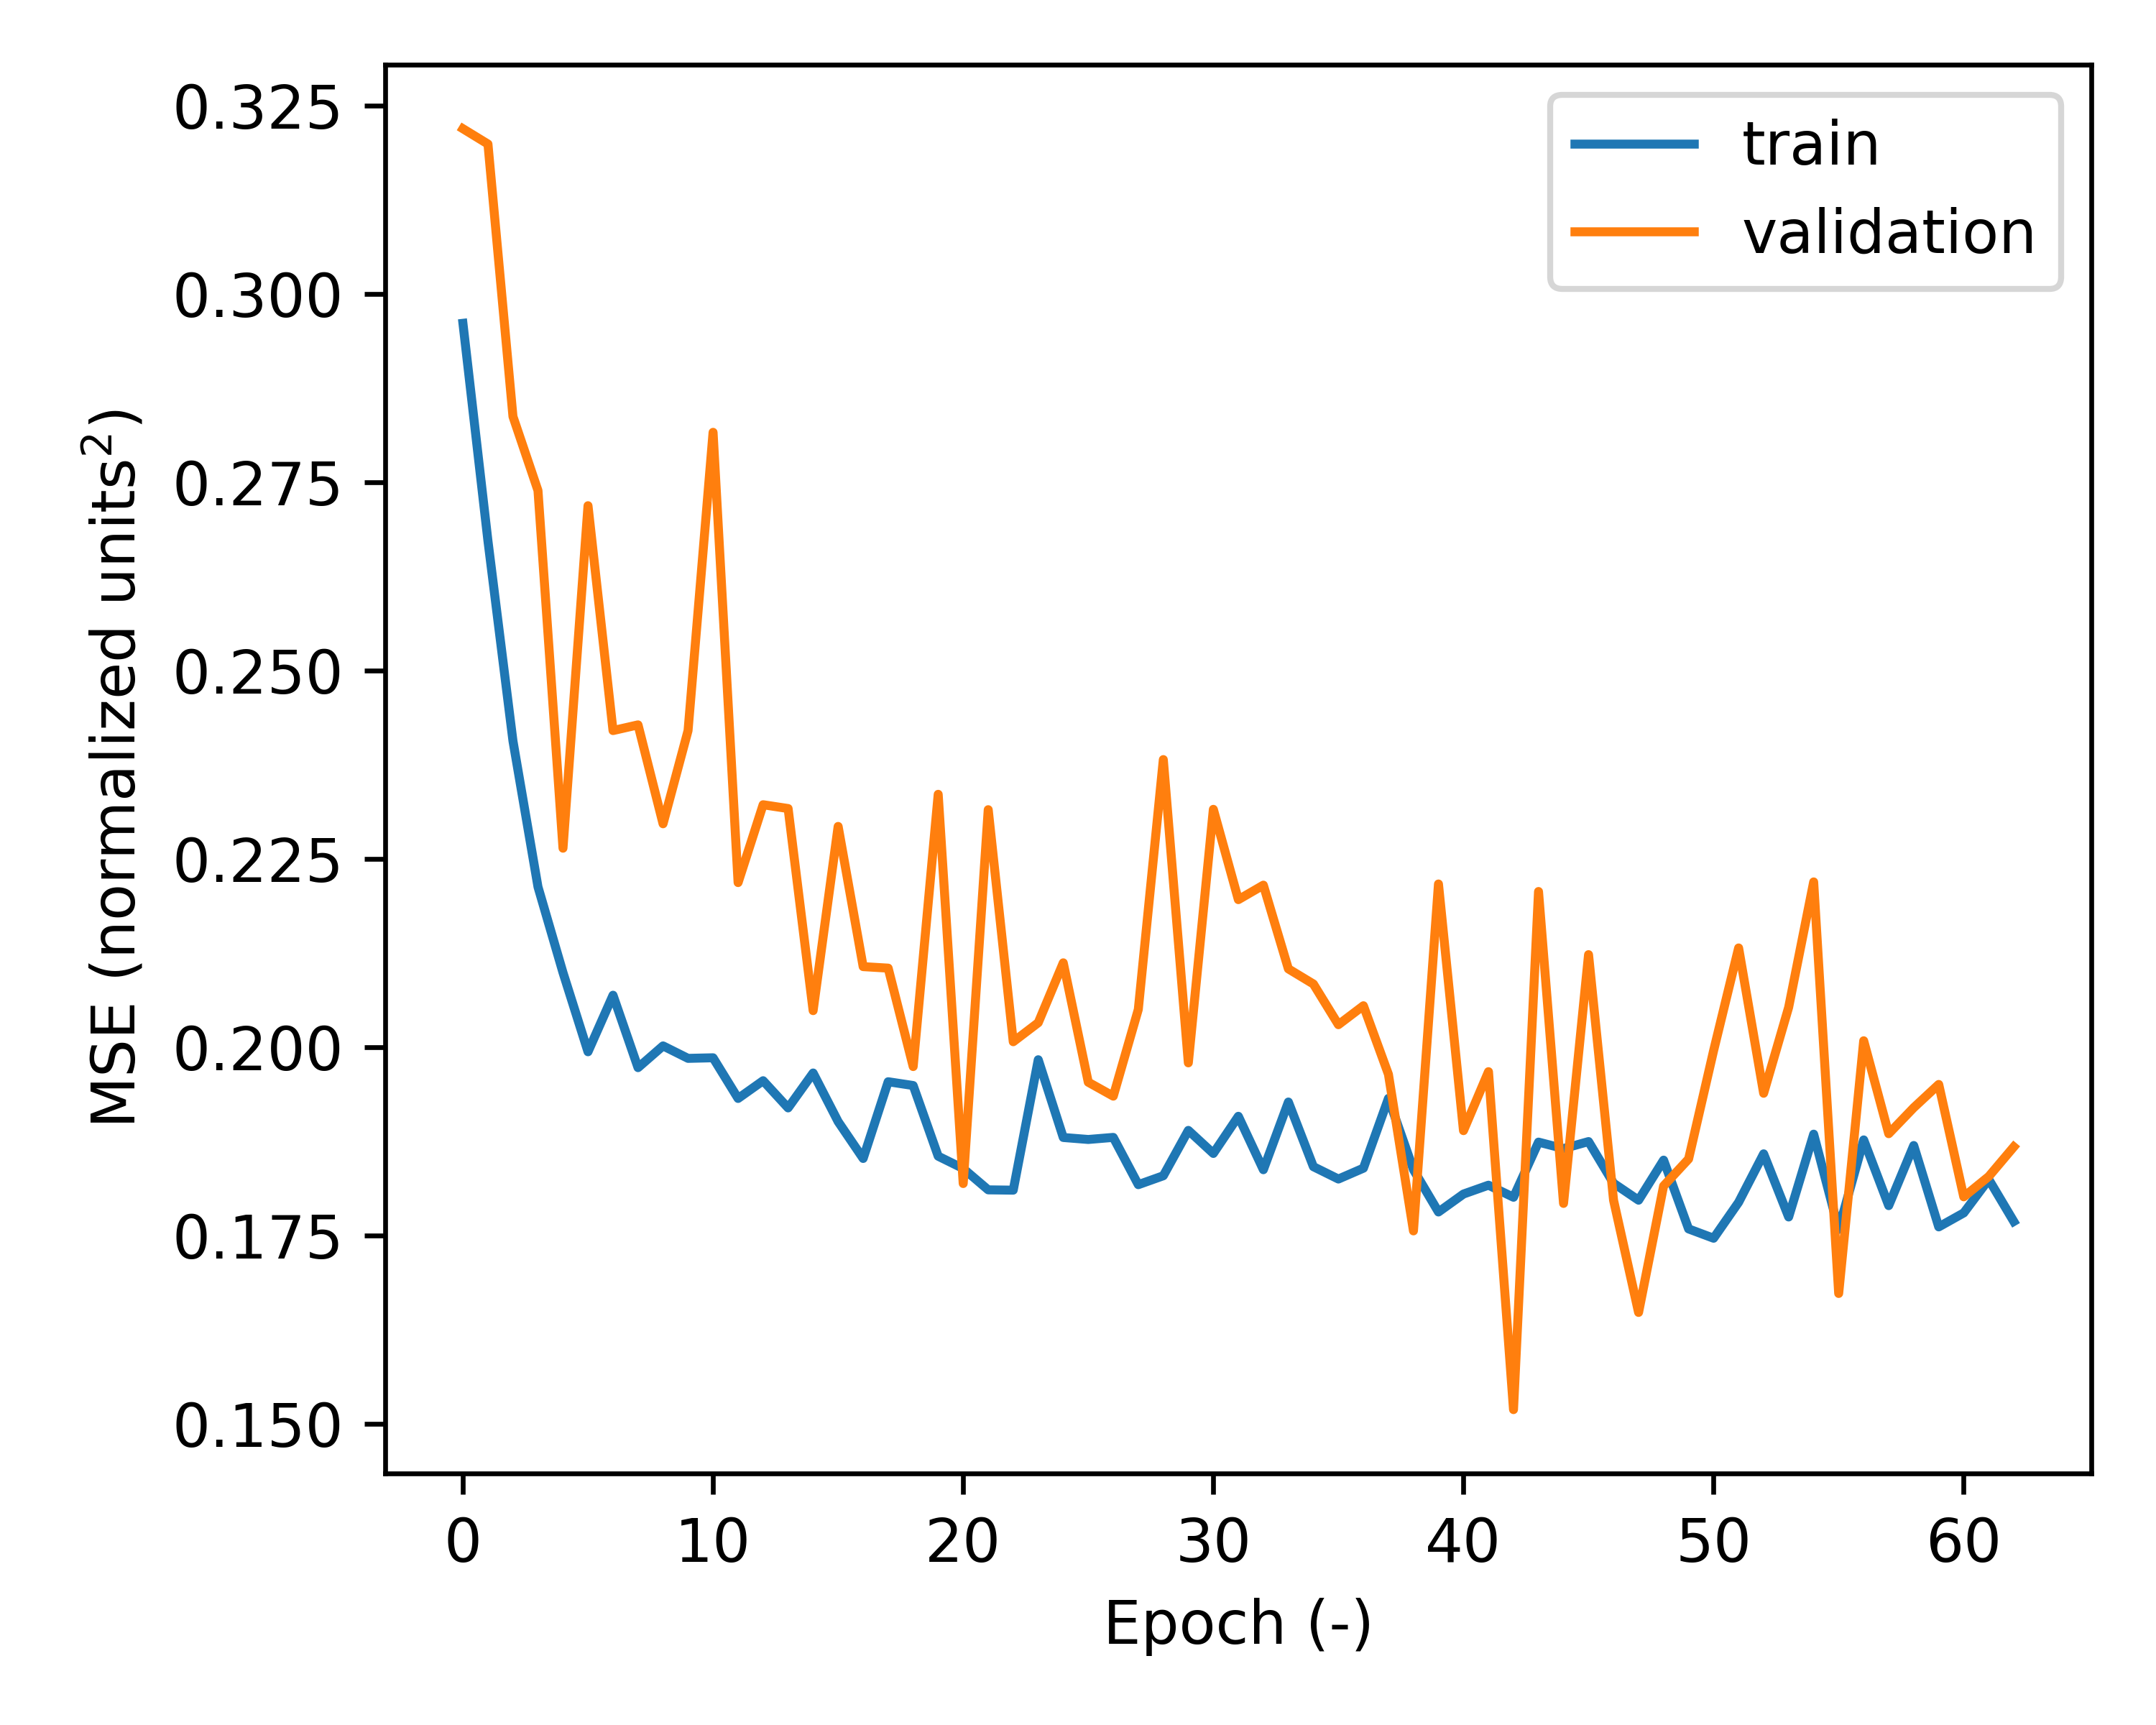
\includegraphics[width=0.46\linewidth]{loss_curve_multi.png}
\caption{Perda de treinamento e validação (MSE) da SNN multimodal selecionada.}
\label{fig:loss_curve_method}
\end{figure}



\FloatBarrier

\section{Configuração da Medição de Energia}

\subsection{Instrumentação e Procedimento}
\textbf{ESP32 e Raspberry Pi:} corrente e tensão foram amostradas a cada 500 ms usando o INA219. Duas janelas foram capturadas: repouso ($N_{idle}$ amostras) e carga ($N_{load}$ amostras) durante a execução do benchmark.\newline
\textbf{Dispositivos Android:} corrente e tensão foram lidas das APIs do sistema sob fases controladas de repouso/carga.
A instrumentação completa e as janelas de amostragem estão resumidas na Tabela~\ref{tab:energy_setup}.

A potência incremental foi estimada como $\Delta P = P_{load} - P_{idle}$, e a energia por inferência como $E_{inf} = \Delta P / \text{vazão}$.

\rev{A Tabela~\ref{tab:android_specs} detalha os três dispositivos Android (A--C) usados na campanha. Como a inferência executa na CPU por meio do interpretador TFLite (XNNPACK, sem delegate de GPU/NNAPI), a configuração dos clusters de CPU e a memória disponível são os recursos relevantes para a carga de IA; as GPUs são listadas apenas por completude.}

\begin{table}[t]
\caption{\rev{Especificações dos dispositivos Android (dados do fabricante; a RAM entre parênteses é o MemTotal reportado pelo sistema).}}
\label{tab:android_specs}
\centering
\scriptsize
\setlength{\tabcolsep}{3pt}
\begin{tabular}{lccc}
\toprule
 & Android A & Android B & Android C \\
\midrule
Aparelho & Redmi Note 12 & Galaxy A56 5G & Redmi Note 11S \\
Modelo & 23021RAAEG & SM-A566E & 2201117SG \\
SoC & Snapdragon 685 & Exynos 1580 & Helio G96 \\
Litografia & 6 nm & 4 nm & 12 nm \\
CPU & 4$\times$A73 2,8 & 1$\times$A720 2,9 & 2$\times$A76 2,05 \\
(GHz) & 4$\times$A53 1,9 & 3$\times$A720 2,6 & 6$\times$A55 2,0 \\
 & & 4$\times$A520 1,95 & \\
GPU & Adreno 610 & Xclipse 540 & Mali-G57 MC2 \\
RAM & 6 GB (5,77) & 8 GB (7,60) & 6 GB (5,86) \\
Android & 15 & 16 & 13 \\
\bottomrule
\end{tabular}
\end{table}

\begin{table}[t]
\caption{Configuração medida e janelas de amostragem por plataforma.}
\label{tab:energy_setup}
\centering
\footnotesize
\setlength{\tabcolsep}{4pt}
\begin{tabular}{lccc}
\toprule
Plataforma & Fonte & $N_{idle}$ & $N_{load}$ \\
\midrule
ESP32 (MicroPy) & INA219 & 50 & 50 \\
Raspberry Pi 4B & INA219 & 97 & 440 \\
Android (A-C) & Telem. sistema & 200 & 200 \\
\bottomrule
\end{tabular}
\end{table}


O envelope de implantação resultante combina vazão e energia incremental por inferência: cenários de alta taxa favorecem a execução em smartphones e SBCs, enquanto o sensoriamento autônomo de baixa taxa ainda pode ser suportado em hardware da classe microcontrolador.

\section{Resultados Experimentais}

\subsection{Desempenho de Predição}
A Tabela~\ref{tab:pred_perf} resume o desempenho macro em um benchmark com múltiplas sementes ($n=10$), reportando média e desvio-padrão. Random Forest e LSTM obtiveram os menores erros médios, enquanto a SNN proposta permaneceu competitiva e substancialmente mais estável que a linha de base MLP.

\begin{table}[!h]
\caption{Desempenho de predição multimodal com múltiplas sementes (métricas macro).}
\label{tab:pred_perf}
\centering
\footnotesize
\setlength{\tabcolsep}{3pt}
\begin{tabular}{lccc}
\toprule
Modelo & MAE macro & RMSE macro & $R^2$ macro \\
\midrule
Random Forest & $\mathbf{0.409 \pm 0.062}$ & $0.557 \pm 0.086$ & $\mathbf{0.335 \pm 0.131}$ \\
LSTM & $0.428 \pm 0.059$ & $\mathbf{0.548 \pm 0.073}$ & $0.313 \pm 0.139$ \\
SNN (proposta) & $0.447 \pm 0.064$ & $0.566 \pm 0.072$ & $0.291 \pm 0.146$ \\
MLP & $0.781 \pm 0.193$ & $0.983 \pm 0.178$ & $-5.460 \pm 5.220$ \\
\bottomrule
\end{tabular}
\end{table}

Embora o Random Forest tenha alcançado o menor MAE, a SNN demonstrou desempenho preditivo competitivo, viabilizando a implantação em dispositivos de borda de baixo consumo, o que é essencial para cenários de monitoramento ambiental remoto. O ranqueamento indica que a SNN não é o modelo de menor erro em termos absolutos, mas permanece em uma faixa competitiva, com robustez materialmente melhor que a do MLP neste regime de poucos dados.

{\sloppy\rev{Para quantificar a incerteza, foram calculados intervalos de confiança de 95\% (distribuição t, $n=10$ sementes) para todas as métricas macro. Para o MAE macro: SNN \mbox{$[0,399;\ 0,495]$}, Random Forest \mbox{$[0,362;\ 0,456]$}, LSTM \mbox{$[0,384;\ 0,472]$} e MLP \mbox{$[0,636;\ 0,926]$}; para o $R^2$ macro: SNN \mbox{$[0,181;\ 0,401]$}, Random Forest \mbox{$[0,237;\ 0,434]$}, LSTM \mbox{$[0,209;\ 0,418]$} e MLP \mbox{$[-9,396;\ -1,524]$}. Os intervalos de SNN, Random Forest e LSTM se sobrepõem substancialmente, enquanto o MLP fica claramente separado.}\par}

\rev{Complementando o teste de sinais reportado na submissão original, testes de Wilcoxon pareados exatos sobre as dez sementes pareadas não mostram diferença significativa entre SNN e Random Forest (MAE \mbox{$p=0,064$}; RMSE \mbox{$p=0,846$}; $R^2$ \mbox{$p=0,922$}) nem entre SNN e LSTM (MAE \mbox{$p=0,105$}; RMSE \mbox{$p=0,131$}; $R^2$ \mbox{$p=0,232$}), enquanto a SNN supera significativamente o MLP em todas as métricas (\mbox{$p=0,002$}). Um teste de Friedman sobre os quatro modelos é significativo (MAE: \mbox{$\chi^2(3)=19,56$}, \mbox{$p<0,001$}), com postos médios de 1,7 (Random Forest), 1,9 (LSTM), 2,4 (SNN) e 4,0 (MLP), confirmando que a diferença global é causada pelo MLP, e não pela separação entre os três modelos líderes.}

\subsection{Desempenho por Alvo}
\rev{A Tabela~\ref{tab:per_target} detalha o comportamento por alvo. Os três modelos líderes alcançam boa predição de pH (\mbox{$R^2 \approx 0,67$}--\mbox{$0,72$}) e erro de turbidez comparável, enquanto o OD exibe $R^2$ médio negativo para todos os modelos, incluindo o Random Forest. Isso é consistente com a análise de correlação da Tabela~\ref{tab:corr_analysis}: o OD é fracamente correlacionado com todos os atributos de entrada disponíveis, de modo que a dificuldade é atribuível ao conjunto de atributos, e não à escolha do modelo.}

\begin{table}[!htbp]
\caption{\rev{MAE e $R^2$ por alvo (média sobre 10 sementes); as células mostram MAE~/~$R^2$.}}
\label{tab:per_target}
\centering
\footnotesize
\setlength{\tabcolsep}{3pt}
\rowcolors{2}{yellow!30}{yellow!30}
\begin{tabular}{lccc}
\toprule
Modelo & pH & OD & TURB \\
\midrule
SNN (proposta) & 0.125 / 0.670 & 0.204 / $-0.162$ & 1.012 / 0.364 \\
Random Forest & 0.097 / 0.715 & 0.203 / $-0.063$ & 0.926 / 0.354 \\
LSTM & 0.112 / 0.673 & 0.203 / $-0.154$ & 0.968 / 0.422 \\
MLP & 0.777 / $-13.39$ & 0.352 / $-3.021$ & 1.214 / 0.032 \\
\bottomrule
\end{tabular}
\end{table}

\subsection{Ablação do Aumento de Dados}
Para quantificar o impacto do aumento de dados, comparamos o treinamento da SNN sem aumento (fator 1) e com aumento $\times 10$ (ruído gaussiano, \mbox{$\sigma=0,01$}) sob o mesmo protocolo em cinco sementes (7, 13, 21, 42, 84). O aumento reduziu o MAE macro de \mbox{$0,496 \pm 0,060$} para \mbox{$0,483 \pm 0,075$} (redução de 2,53\%), com leve melhora do $R^2$ macro (\mbox{$0,254 \rightarrow 0,256$}) e RMSE macro praticamente inalterado (\mbox{$0,615 \rightarrow 0,617$}). O ganho por alvo mais relevante foi no MAE de turbidez (\mbox{$1,139 \rightarrow 1,102$}), apoiando o aumento de dados como estratégia prática de estabilização para este tamanho de conjunto.

\subsection{Sensibilidade aos Pesos dos Alvos}
Como a turbidez é o alvo mais difícil, também avaliamos uma pequena varredura de pesos da perda na SNN para quantificar o compromisso entre ajuste global e otimização focada em TURB. A Tabela~\ref{tab:snn_weight_sweep_sba} mostra que aumentar o peso de TURB pode reduzir o $MAE_{TURB}$, mas com leve queda do $R^2$ global.

\begin{table}[!htbp]
\caption{Varredura de pesos da perda na SNN (10 sementes).}
\label{tab:snn_weight_sweep_sba}
\centering
\footnotesize
\setlength{\tabcolsep}{3pt}
\begin{tabular}{lccc}
\toprule
Pesos (pH, OD, TURB) & MAE macro & MAE TURB & $R^2$ macro \\
\midrule
\mbox{$(0.20,\,0.20,\,0.60)$} & $\mathbf{0.447}$ & $1.012$ & $\mathbf{0.291}$ \\
\mbox{$(0.15,\,0.15,\,0.70)$} & $0.452$ & $1.022$ & $0.289$ \\
\mbox{$(0.10,\,0.10,\,0.80)$} & $0.454$ & $1.028$ & $0.288$ \\
\mbox{$(0.05,\,0.15,\,0.80)$} & $0.448$ & $\mathbf{1.006}$ & $0.280$ \\
\bottomrule
\end{tabular}
\end{table}

\subsection{Comportamento Predito vs.\ Real}
A Figura~\ref{fig:pred_true_multi_sba} complementa as métricas agregadas mostrando a concordância ponto a ponto entre valores preditos e observados para cada alvo. pH e OD concentram-se mais próximos da linha de identidade, enquanto a turbidez apresenta maior dispersão, de forma consistente com sua maior contribuição de erro nas tabelas anteriores. \rev{Para o OD em particular, a concordância visual deve ser lida em conjunto com a Tabela~\ref{tab:per_target}: a baixa variância do OD no conjunto de dados (Tabela~\ref{tab:dataset_stats}) mantém os erros absolutos pequenos, mas a fraca correlação entrada--alvo limita a variância explicada para todos os modelos avaliados, e não apenas para a SNN.}

\begin{figure*}[!t]
\centering
\begin{minipage}{0.21\textwidth}
\centering
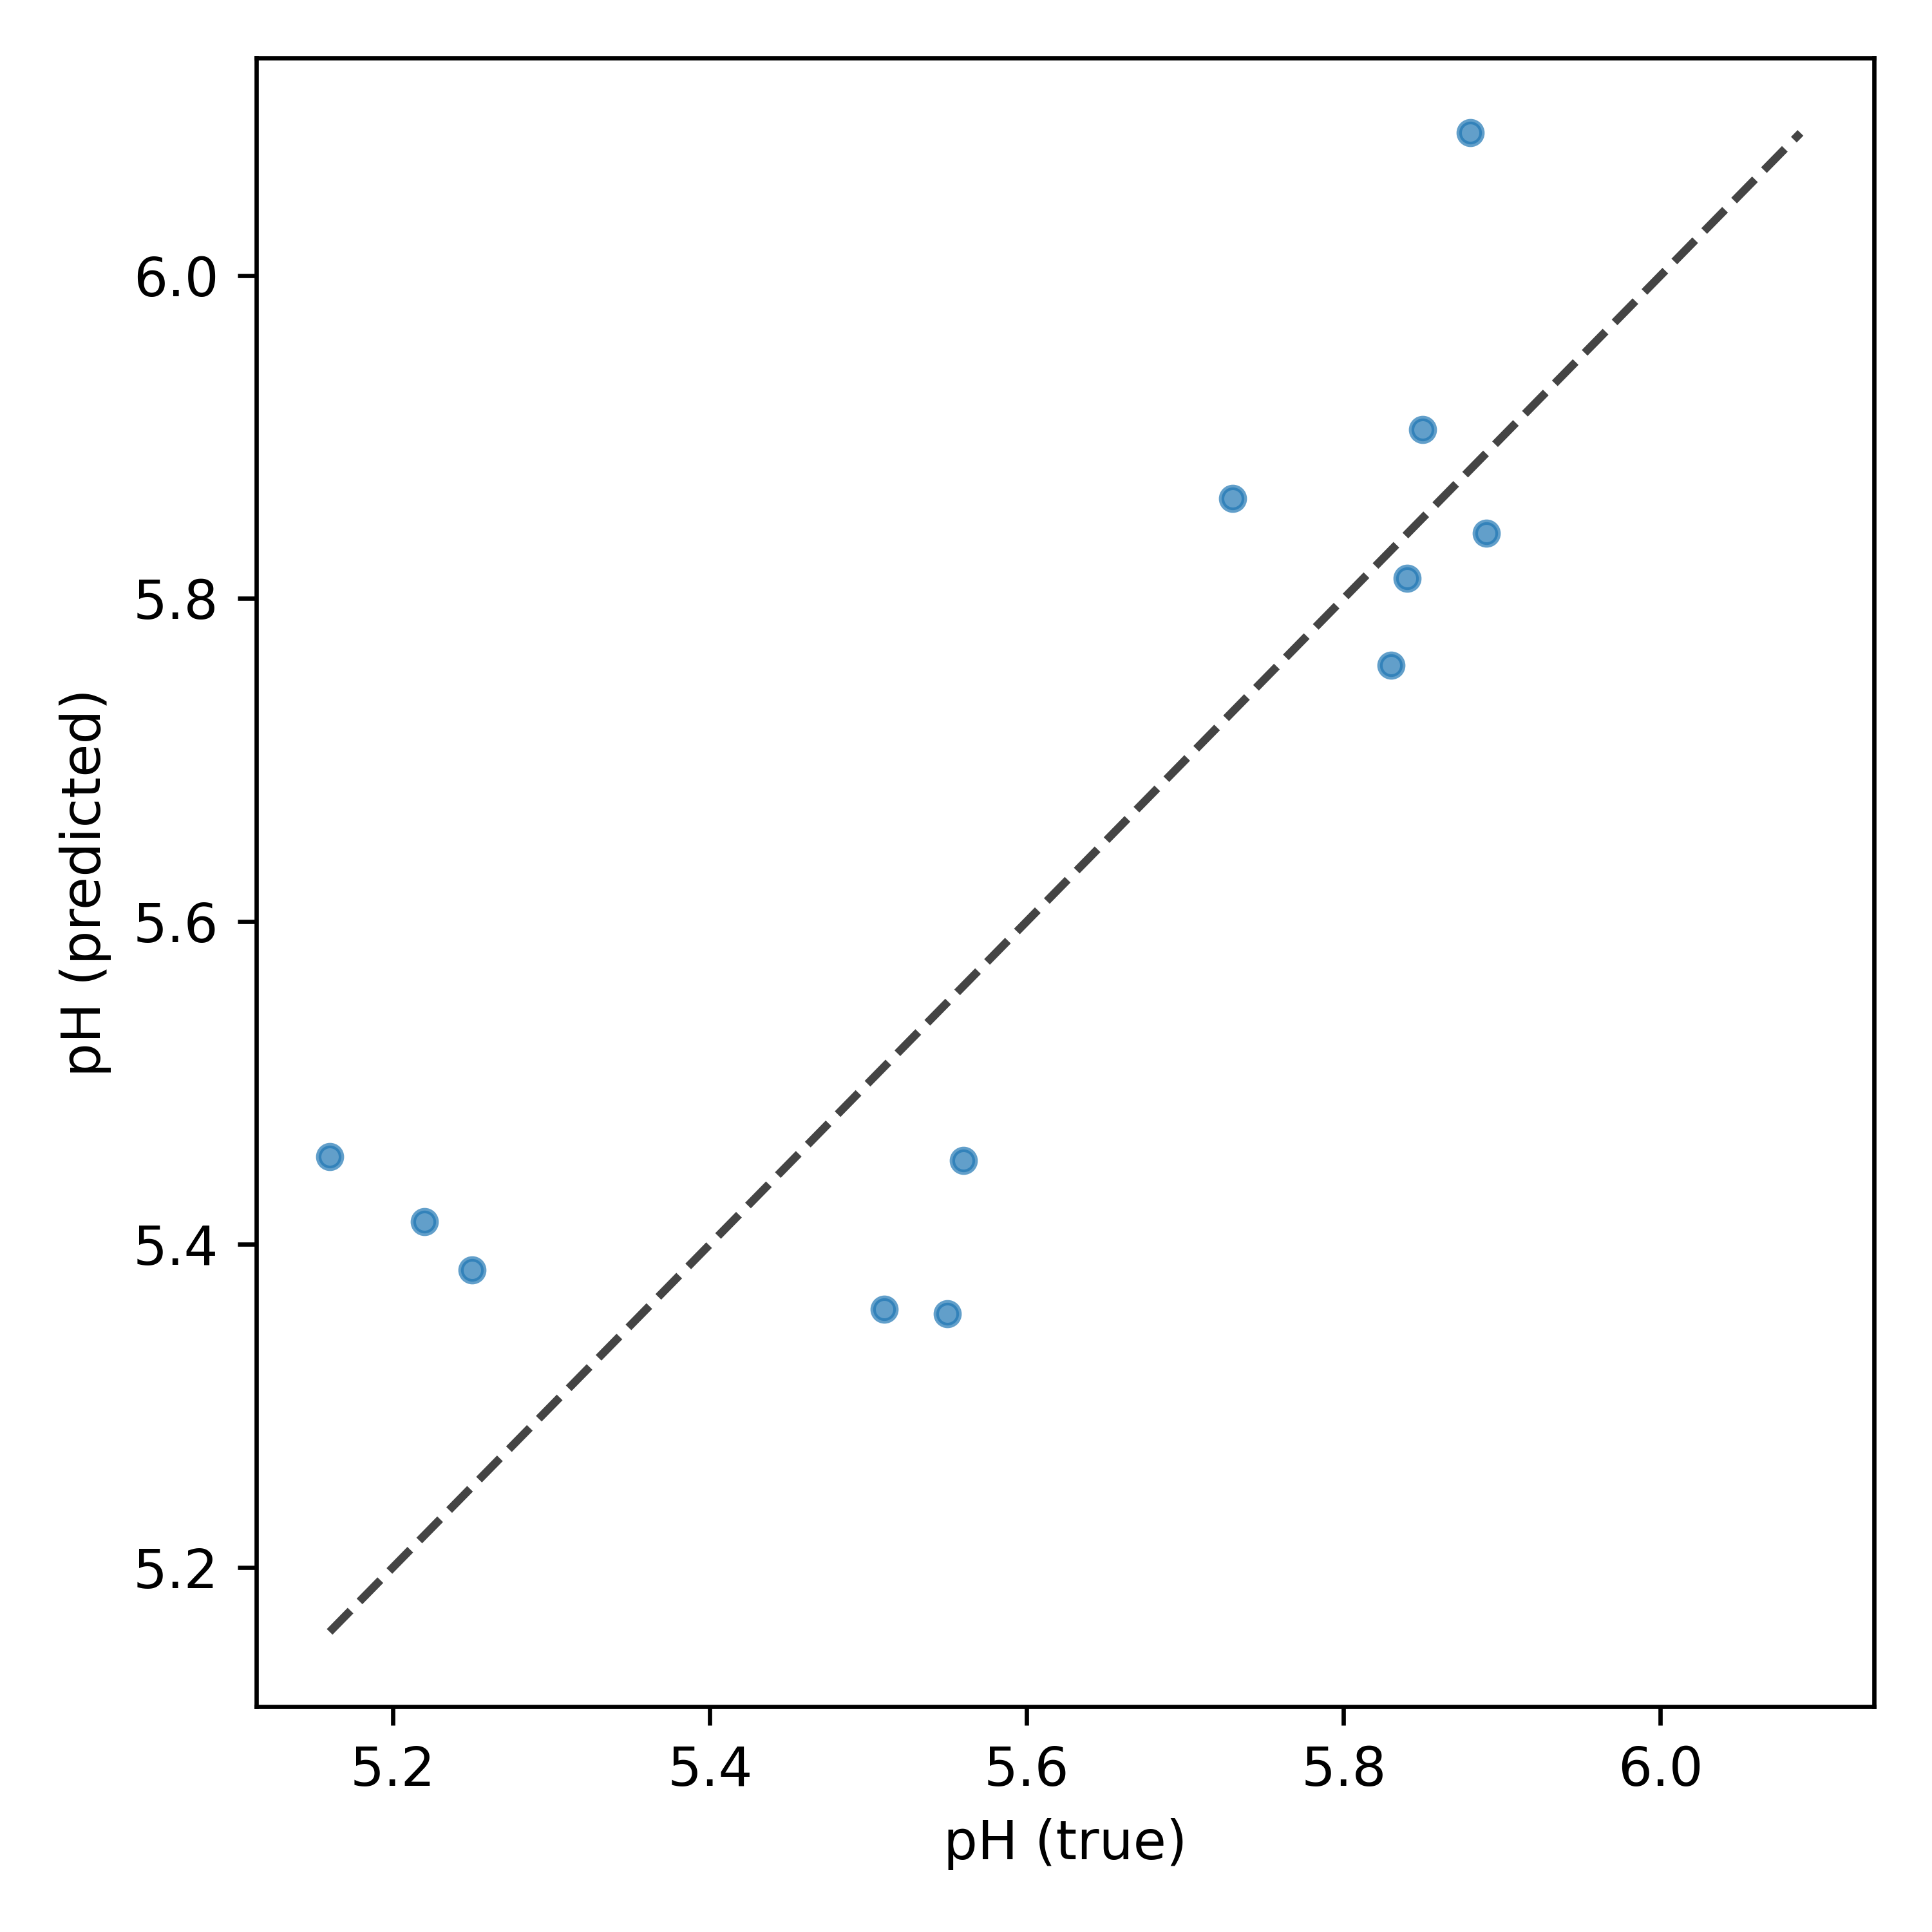
\includegraphics[width=\linewidth]{pred_vs_real_pH_multi.png}
\par\vspace{1mm}{\footnotesize (a) pH\par}
\end{minipage}\hspace{6mm}
\begin{minipage}{0.21\textwidth}
\centering
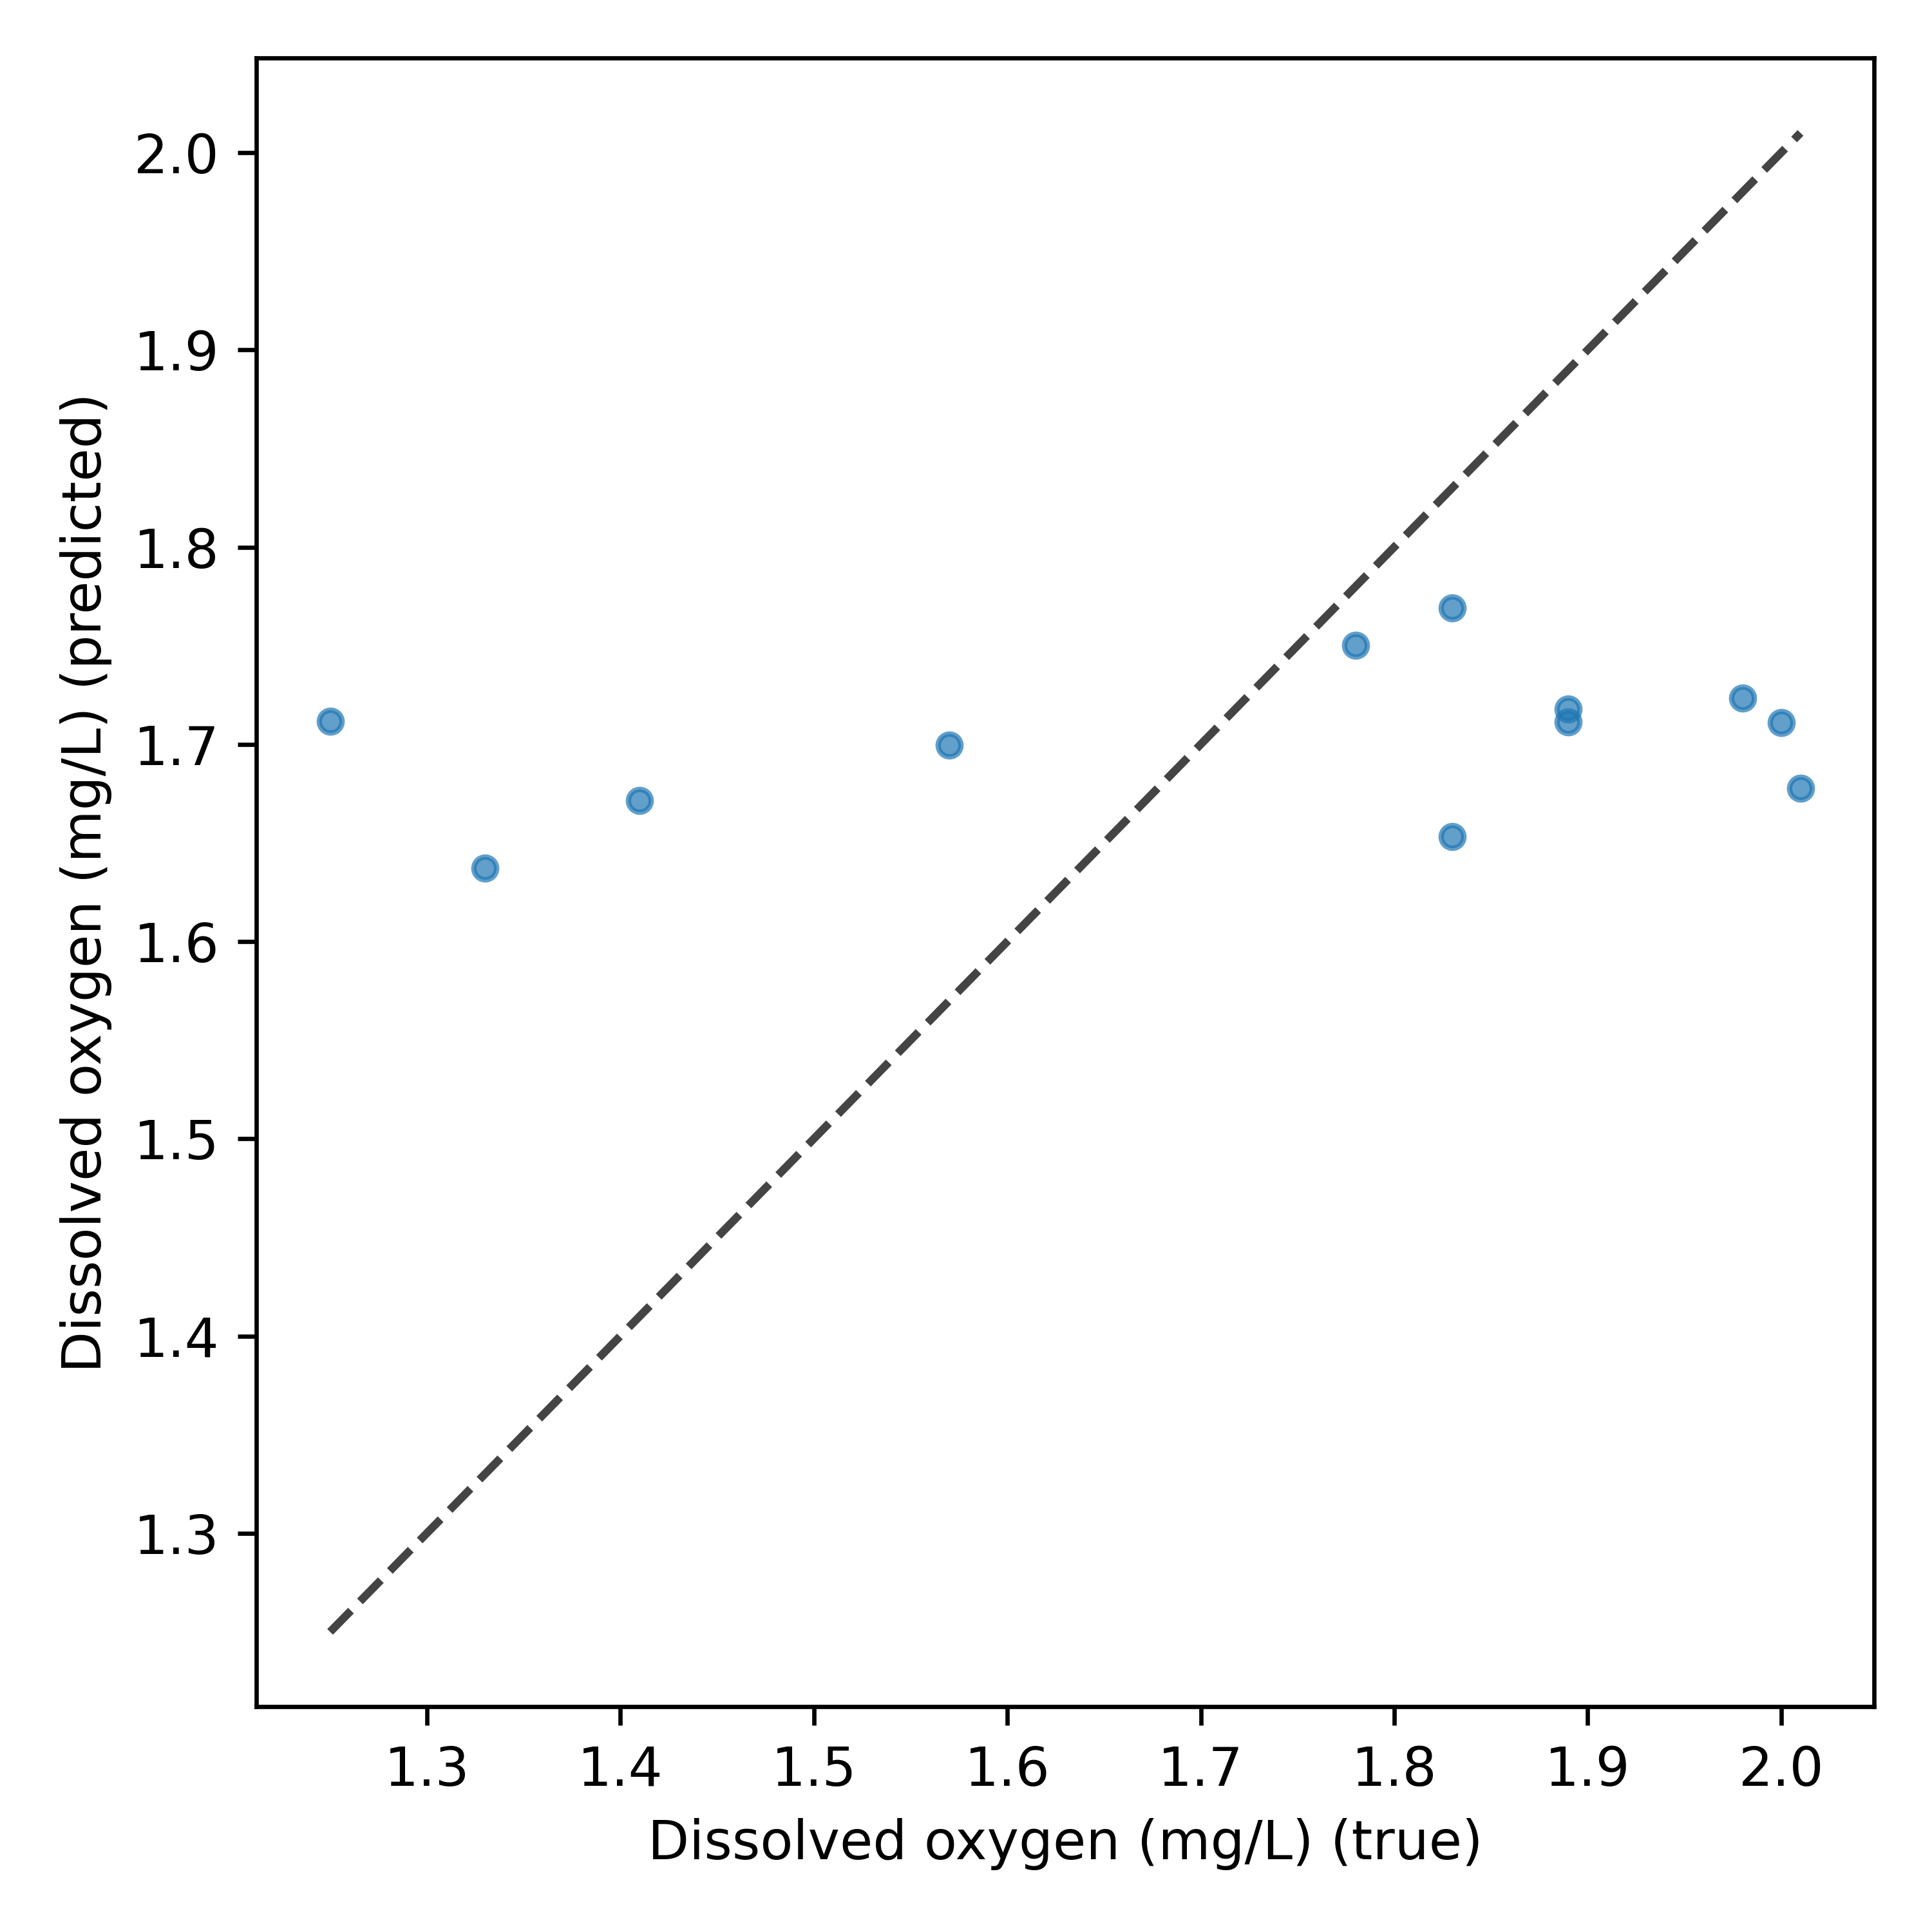
\includegraphics[width=\linewidth]{pred_vs_real_OD_multi.png}
\par\vspace{1mm}{\footnotesize (b) OD\par}
\end{minipage}\hspace{6mm}
\begin{minipage}{0.21\textwidth}
\centering
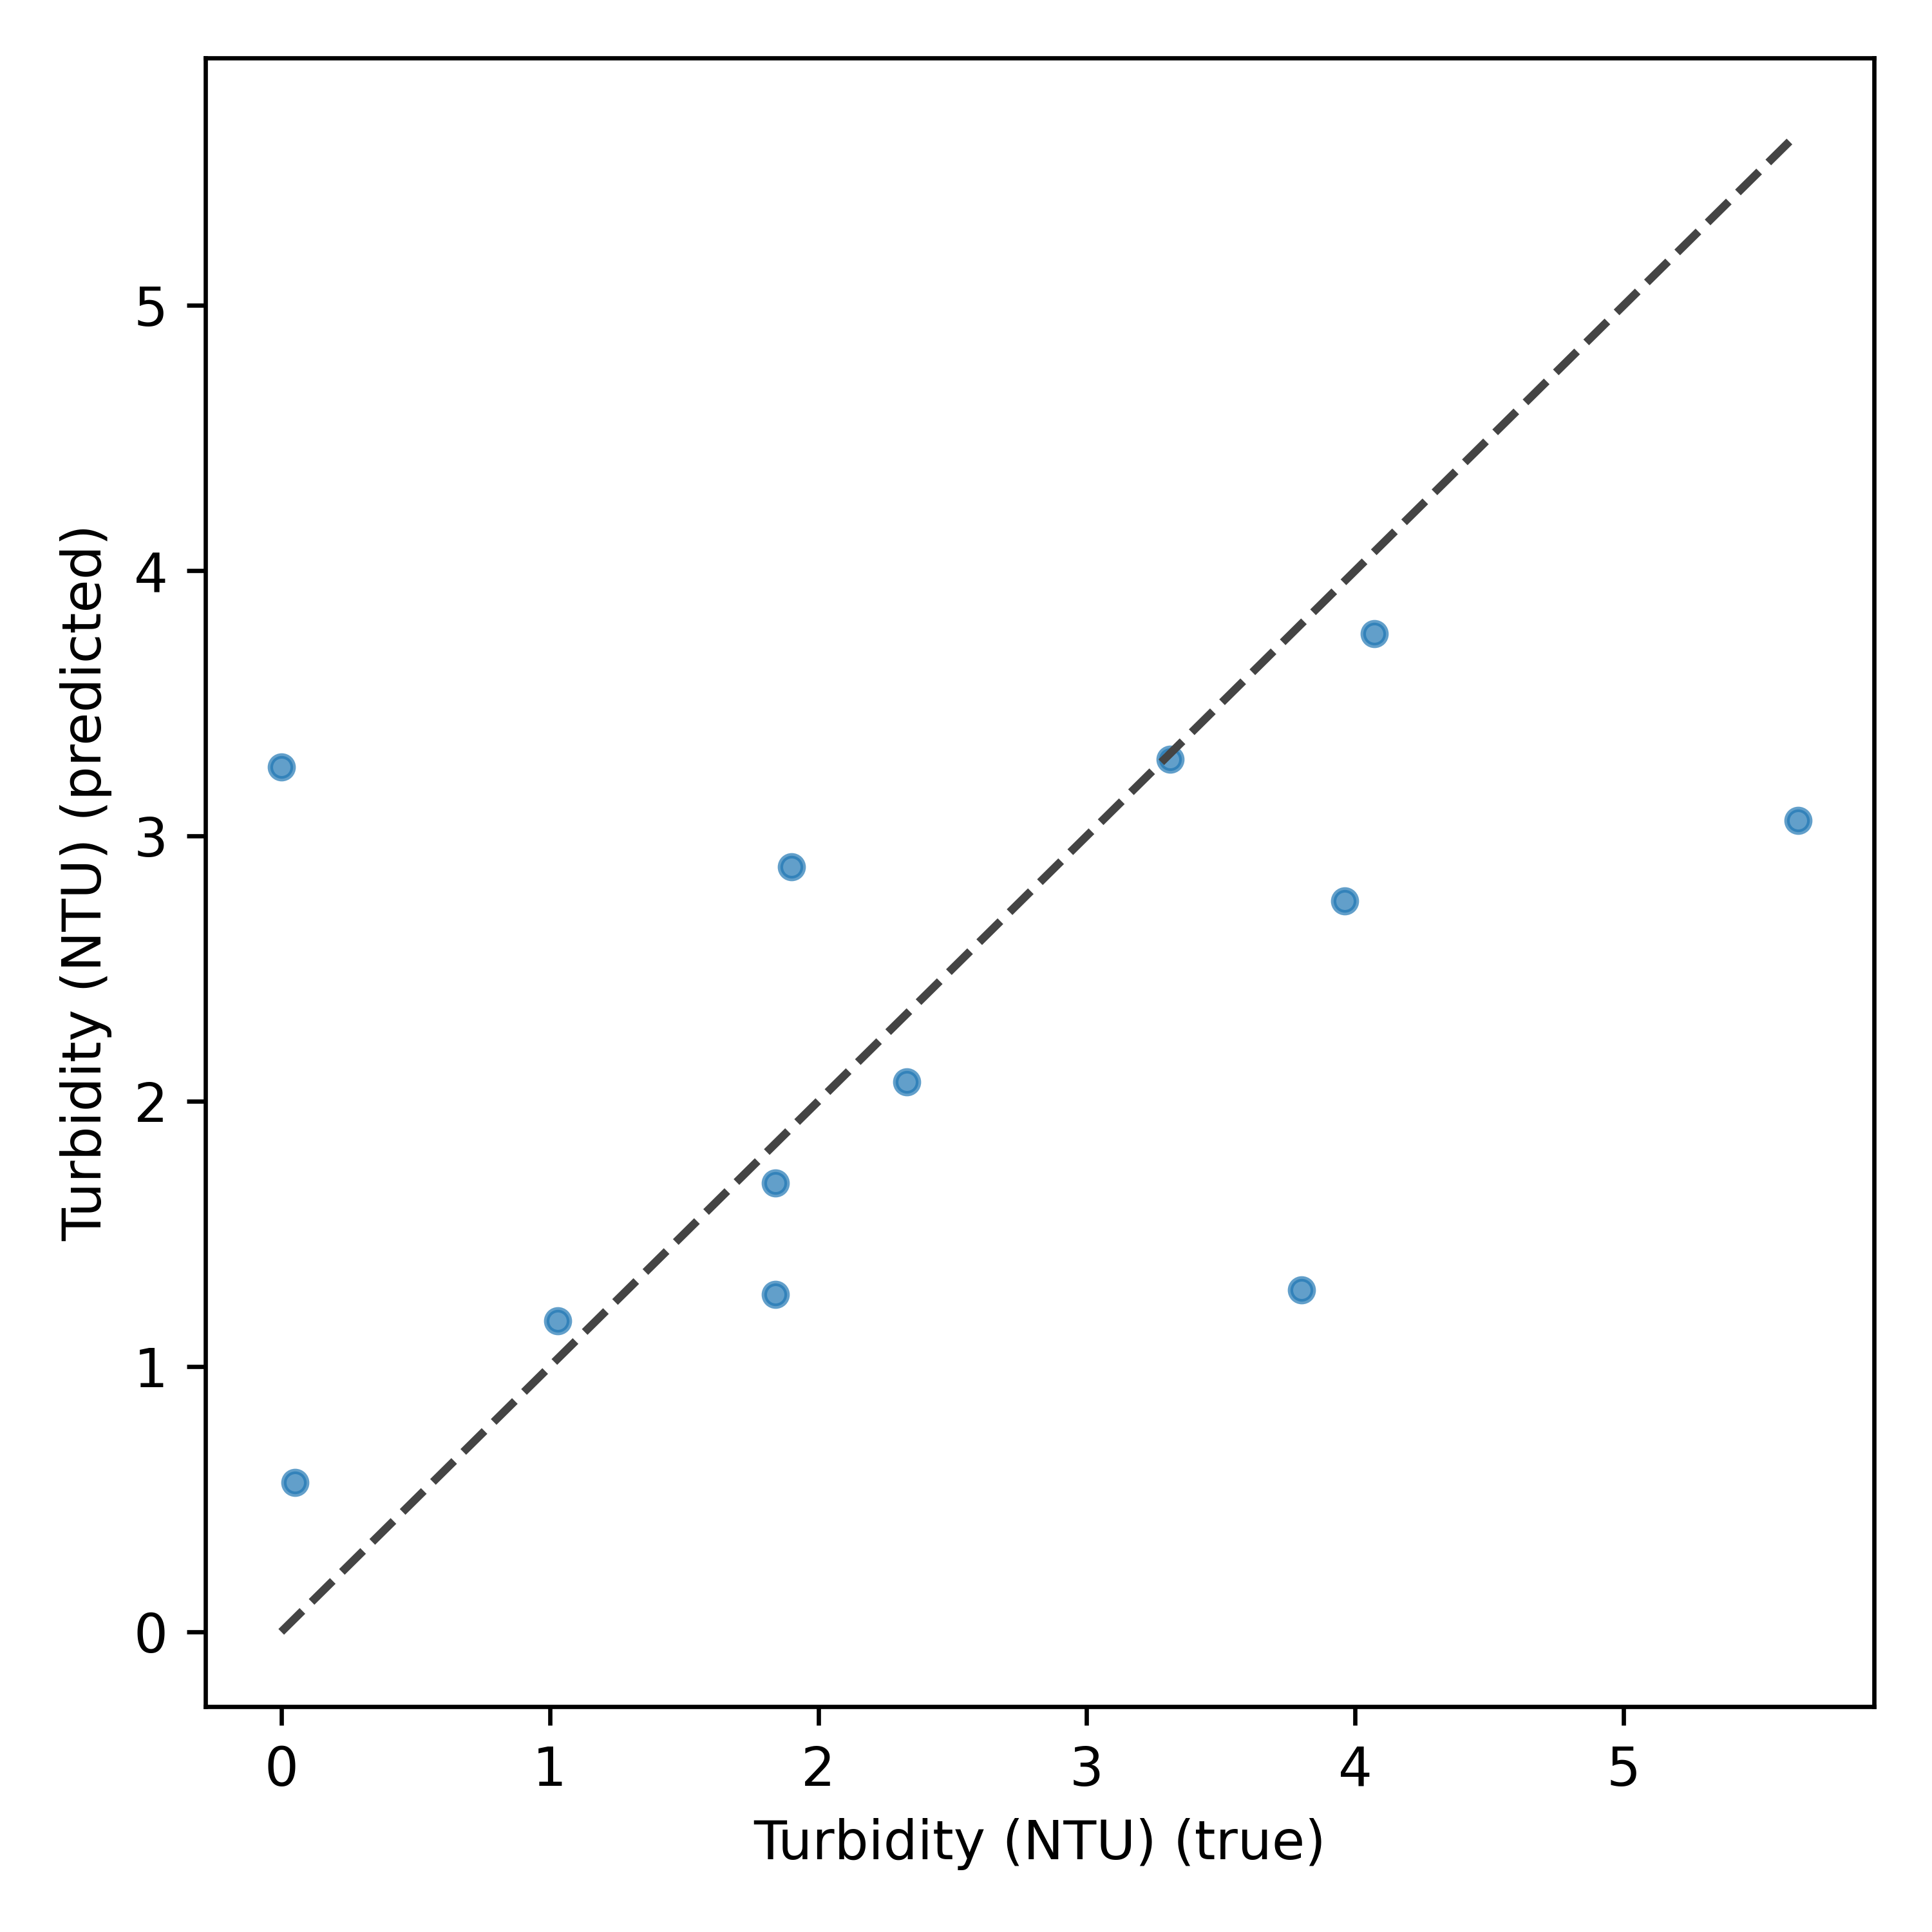
\includegraphics[width=\linewidth]{pred_vs_real_TURB_multi.png}
\par\vspace{1mm}{\footnotesize (c) TURB\par}
\end{minipage}
\caption{Valores preditos vs.\ reais na SNN multimodal para pH, oxigênio dissolvido e turbidez. \rev{(Figura ampliada para a largura total da página nesta revisão, para legibilidade dos eixos.)}}
\label{fig:pred_true_multi_sba}
\end{figure*}

\subsection{Resultados Espaciais e Índice de Poluição}
A interpolação IDW foi usada para converter predições pontuais em superfícies espaciais contínuas, melhorando a interpretação ambiental para além das métricas pontuais. Como mostra a Figura~\ref{fig:idw_combined_sba}, os mapas resultantes evidenciam comportamento espacial não uniforme de pH, oxigênio dissolvido e turbidez, e indicam microzonas candidatas para inspeção de campo priorizada.

\begin{figure*}[!t]
\centering
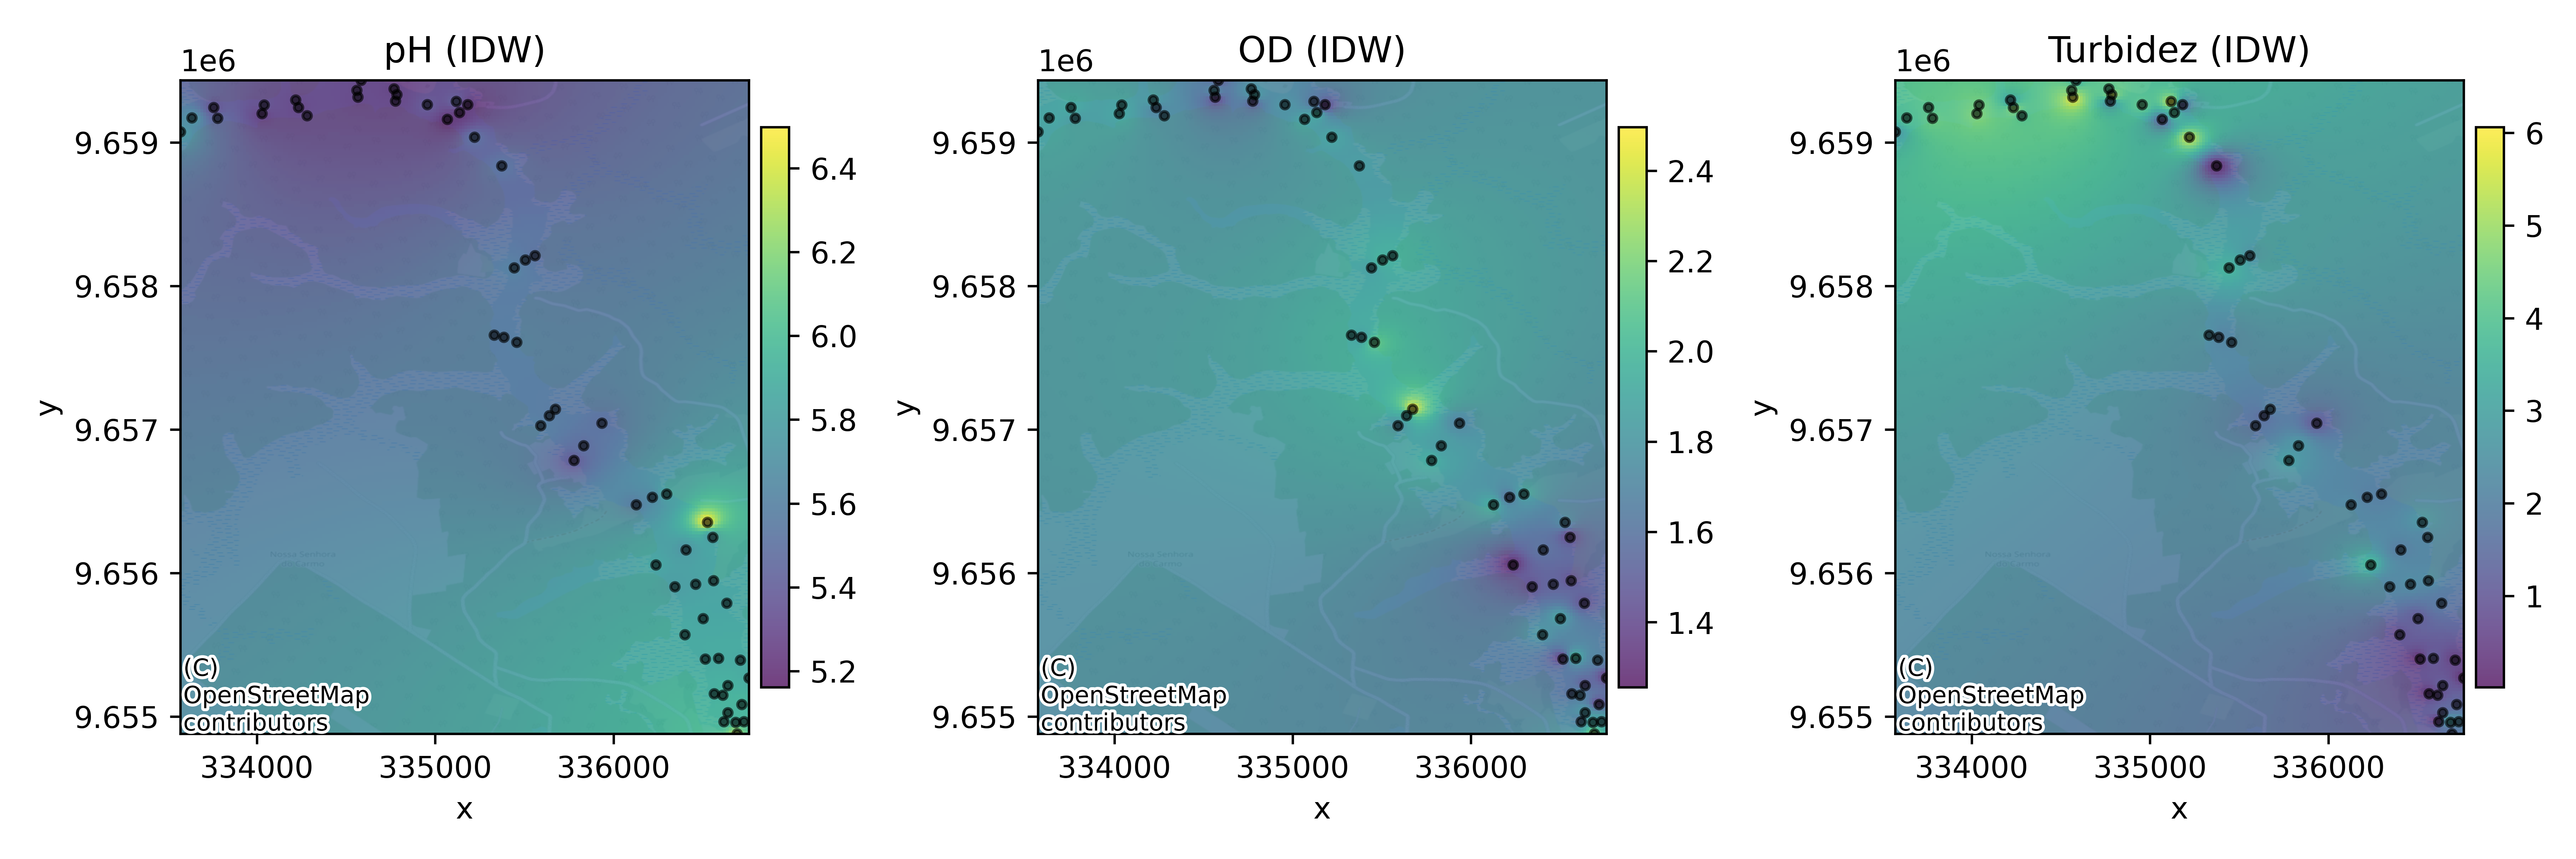
\includegraphics[width=0.70\textwidth]{idw_combined.png}
\caption{Superfícies interpoladas por IDW para pH, oxigênio dissolvido e turbidez a partir dos pontos amostrados. \rev{(Figura ampliada para a largura total da página nesta revisão, para legibilidade dos eixos.)}}
\label{fig:idw_combined_sba}
\end{figure*}

Para apoiar a triagem operacional, um índice composto de poluição foi calculado a partir das predições multimodais e normalizado para \mbox{$[0,1]$}, em que valores mais altos indicam pior condição relativa dentro do conjunto analisado. Como ilustra a Figura~\ref{fig:pollution_sba}, a representação em nível de ponto e sua estimativa espacial por IDW sobre o mapa-base OSM fornecem uma ferramenta visual direta para a identificação de áreas críticas.

\begin{figure*}[!t]
\centering
\begin{minipage}[t]{0.28\textwidth}
\centering
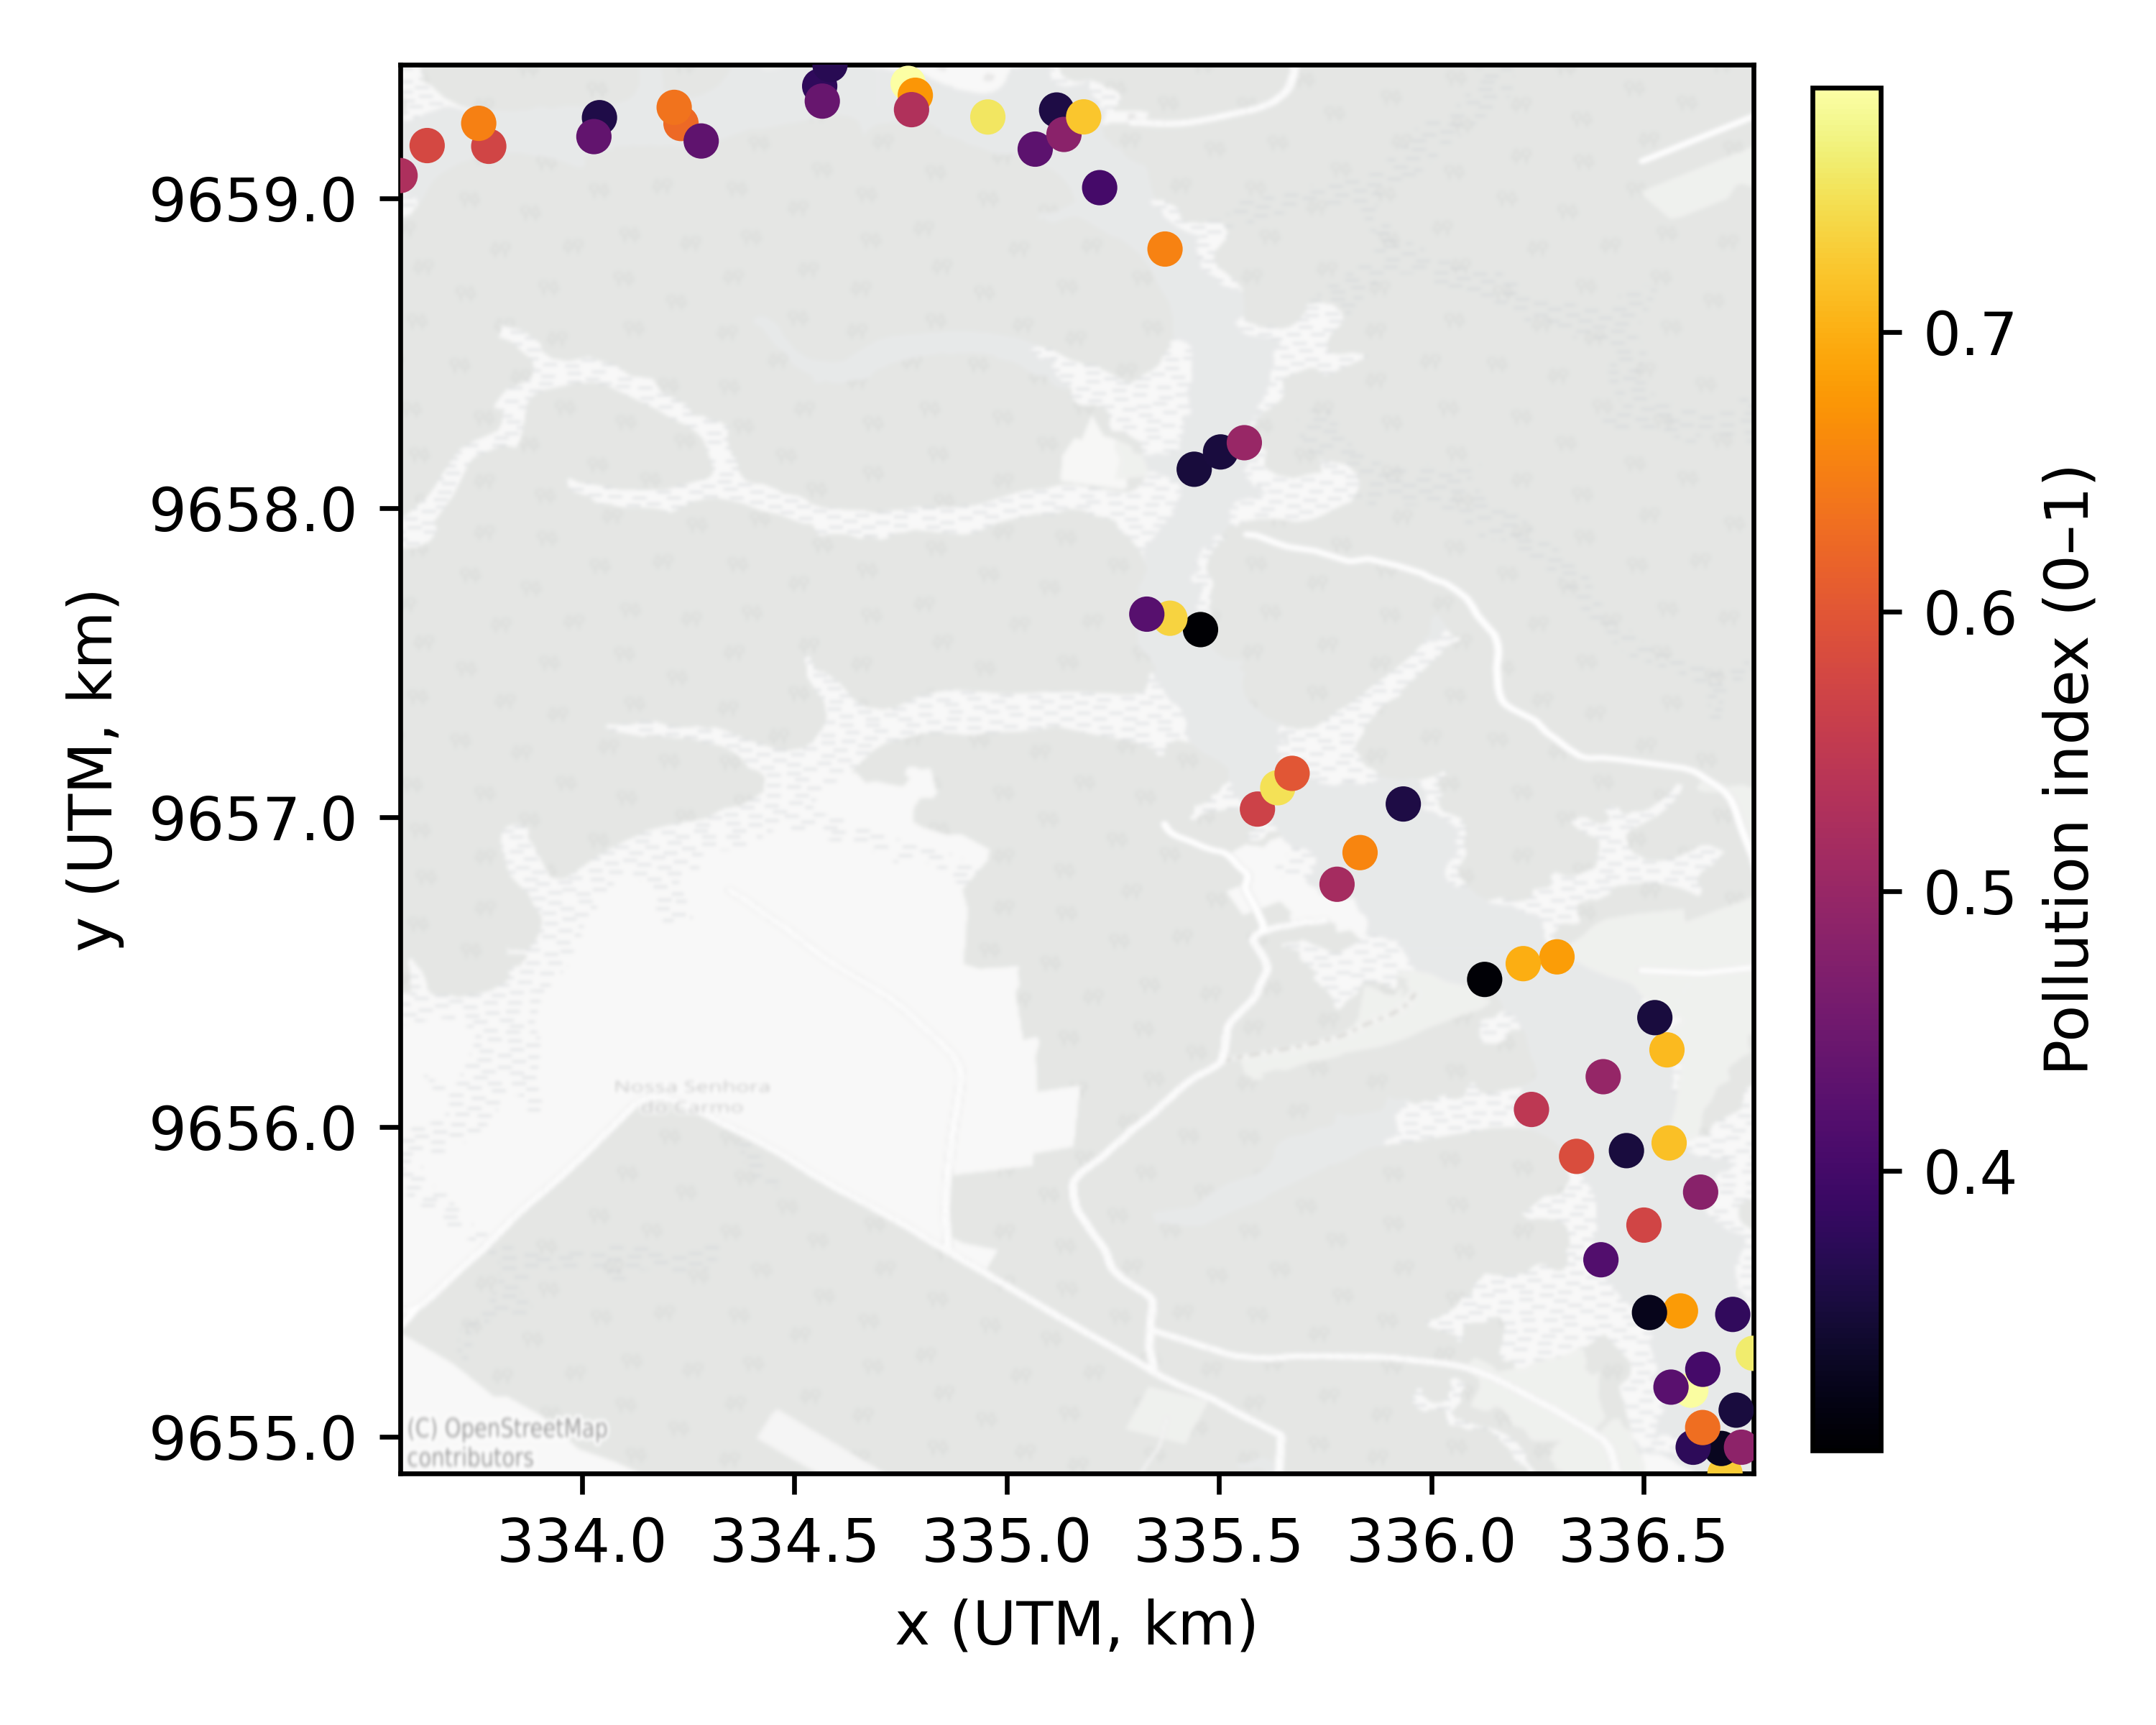
\includegraphics[width=\linewidth]{pollution_scatter.png}
\par\vspace{1mm}{\footnotesize (a) Índice de poluição nos pontos amostrados.\par}
\end{minipage}\hspace{8mm}
\begin{minipage}[t]{0.28\textwidth}
\centering
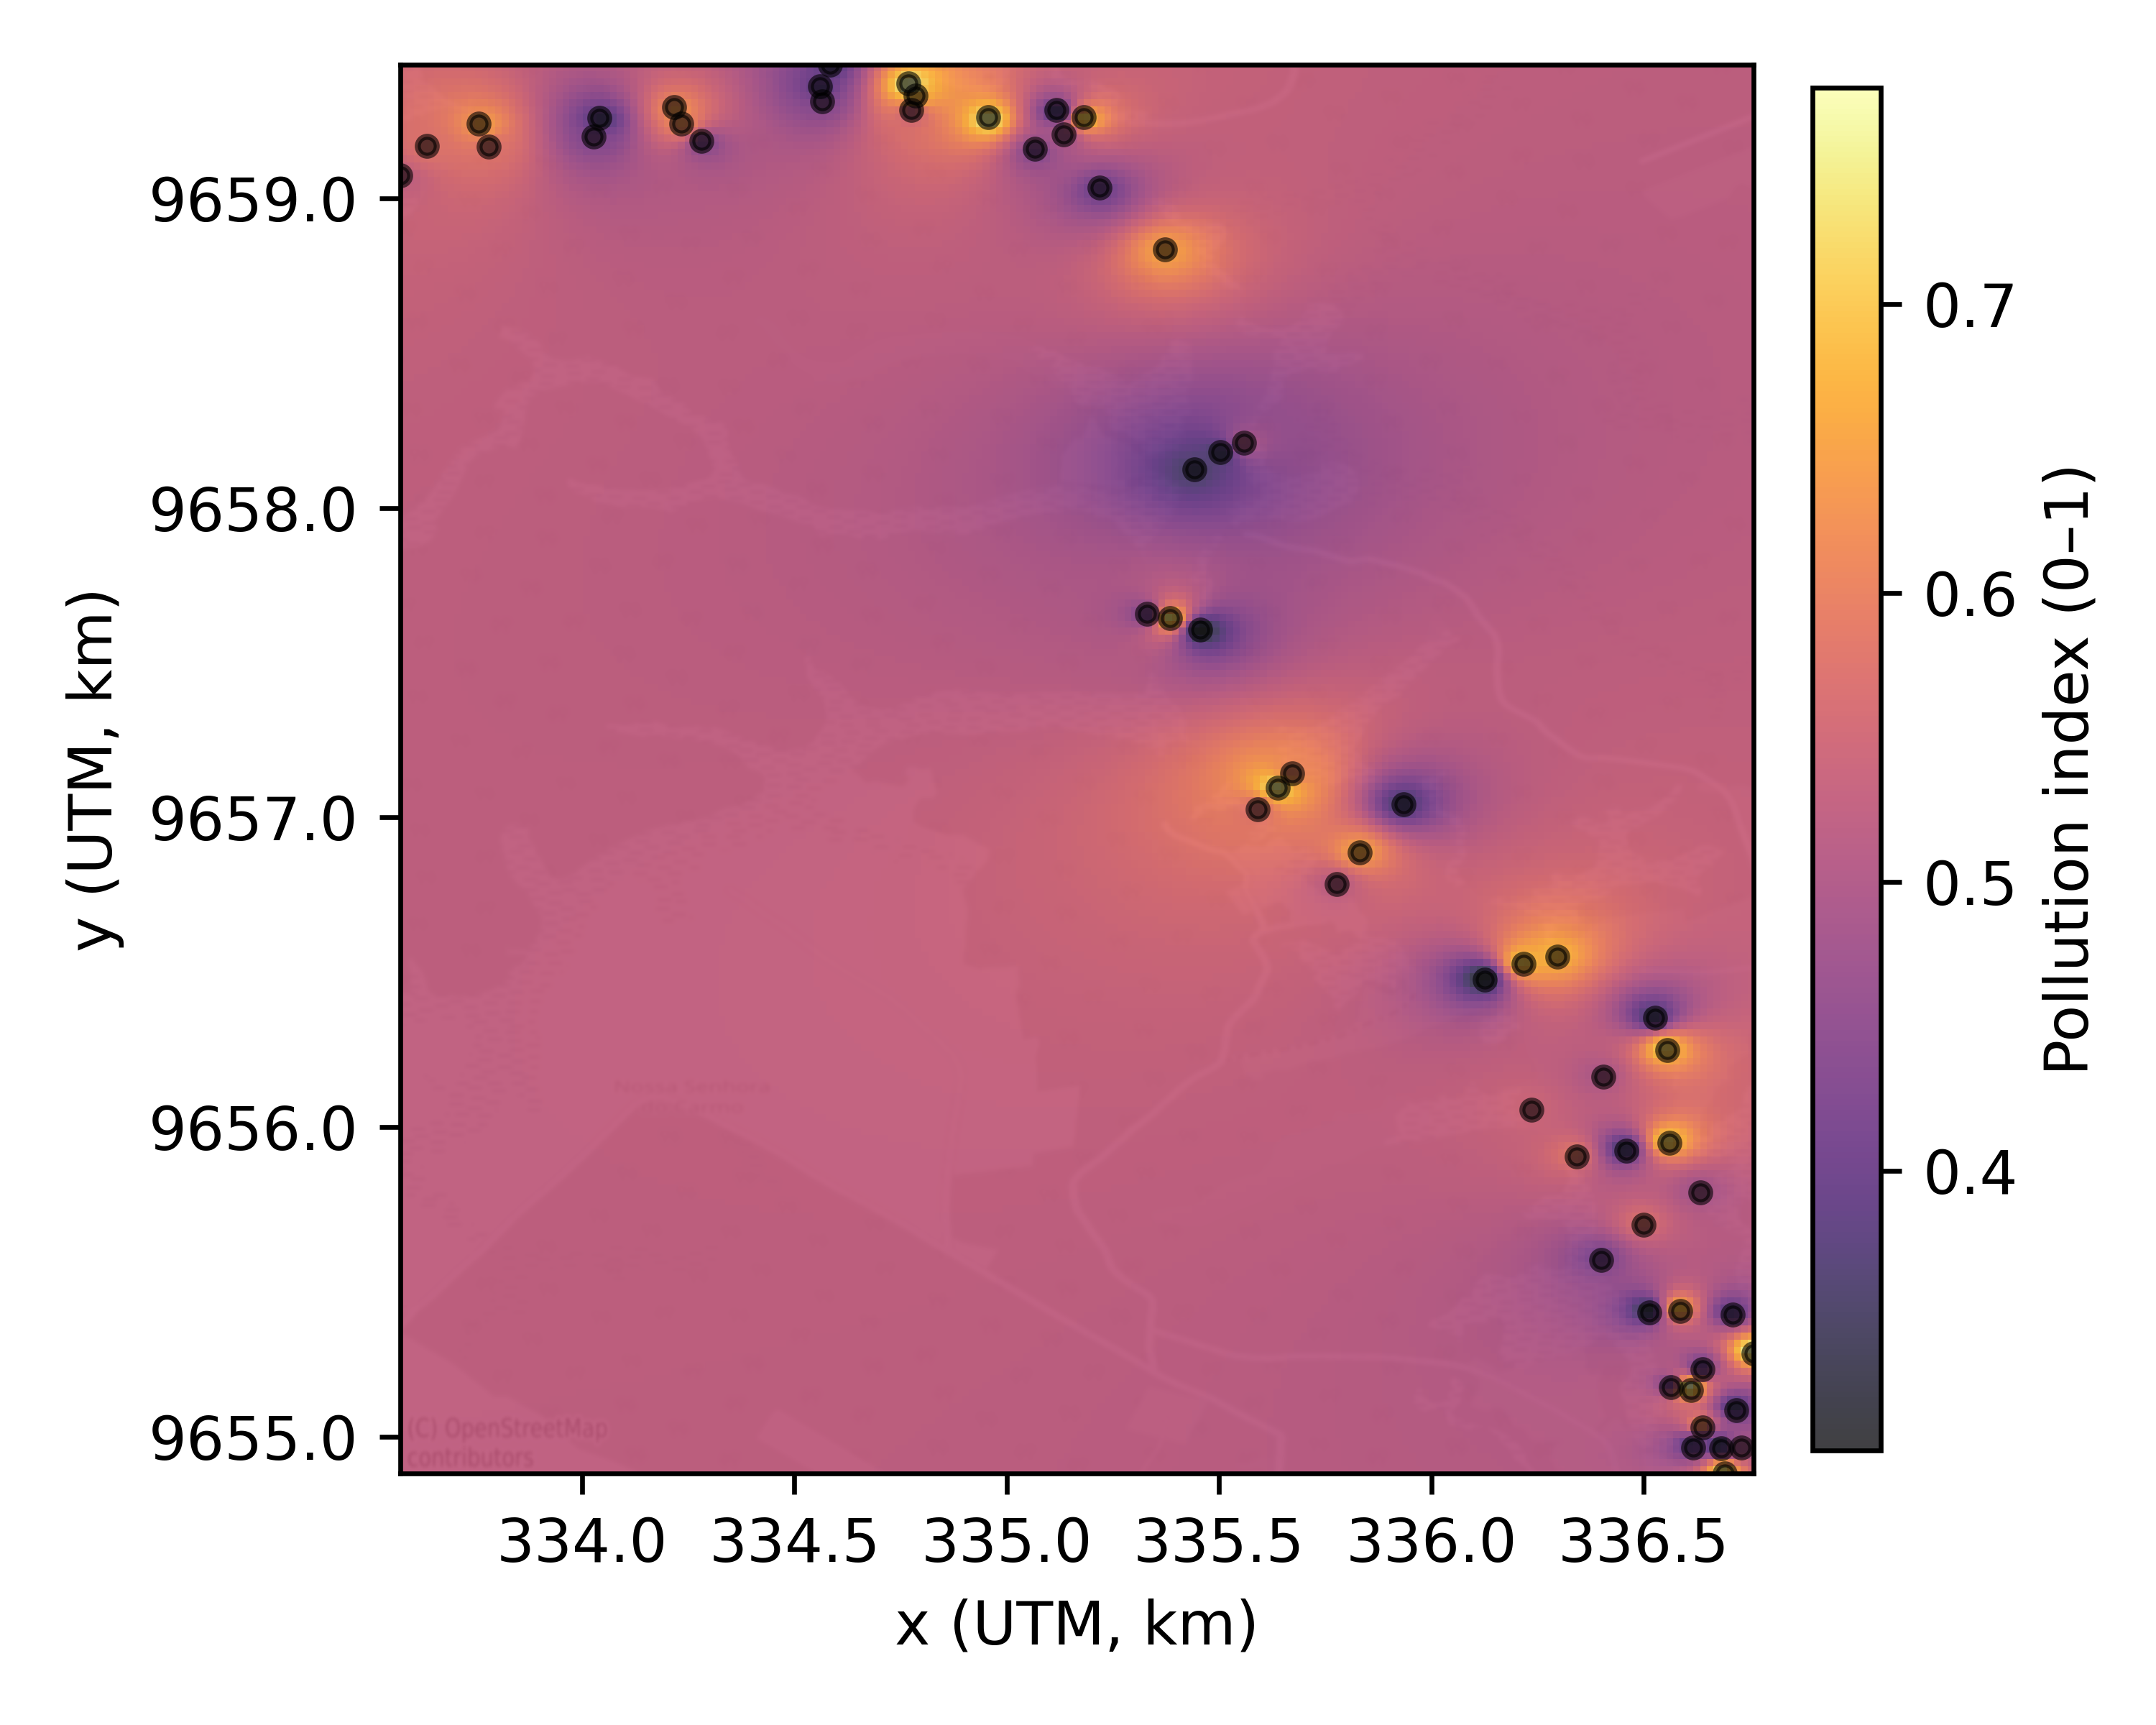
\includegraphics[width=\linewidth]{pollution_idw.png}
\par\vspace{1mm}{\footnotesize (b) Superfície IDW do índice.\par}
\end{minipage}
\caption{Estimativa espacial do índice composto de poluição a partir das predições multimodais (escala normalizada $[0, 1]$) sobre mapa-base OpenStreetMap (UTM 21S). \rev{(Figura ampliada para a largura total da página nesta revisão, para legibilidade dos eixos.)}}
\label{fig:pollution_sba}
\end{figure*}

\subsection{Consumo de Energia e Latência}
A Tabela~\ref{tab:energy_latency} reporta a energia incremental por inferência e a vazão nas plataformas de implantação. O ESP32 é viável para cenários autônomos de baixa taxa, mas apresenta maior energia por inferência devido à vazão limitada. Raspberry Pi e dispositivos Android fornecem mJ/inf muito menores em configurações de alta vazão.

\begin{table}[!htbp]
\caption{Latência/vazão e energia incremental nas plataformas.}
\label{tab:energy_latency}
\centering
\footnotesize
\setlength{\tabcolsep}{3pt}
\begin{tabular}{lccc}
\toprule
Plataforma & Vazão (amostras/s) & $\Delta P$ (W) & $E$ (mJ/inf) \\
\midrule
ESP32 (MicroPy) & 5.0 & 0.056 & 11.204 \\
Raspberry Pi 4B & 4670.50 & 0.239 & 0.0512 \\
Android A & 12337.40 & 0.128 & 0.0104 \\
Android B & 30905.08 & 0.468 & 0.0151 \\
Android C & 16121.71 & 0.046 & 0.00285 \\
\bottomrule
\end{tabular}
\end{table}

A Figura~\ref{fig:energy_bar_lnncs} compara a energia incremental por inferência em escala logarítmica: o ESP32 tem o maior custo por predição, principalmente devido à baixa vazão, enquanto Raspberry Pi e dispositivos Android operam em uma faixa de mJ/inf muito menor; maior vazão nem sempre implica menor energia por inferência, de modo que a seleção de plataforma deve considerar conjuntamente velocidade e potência incremental.

\begin{figure}[!htbp]
\centering
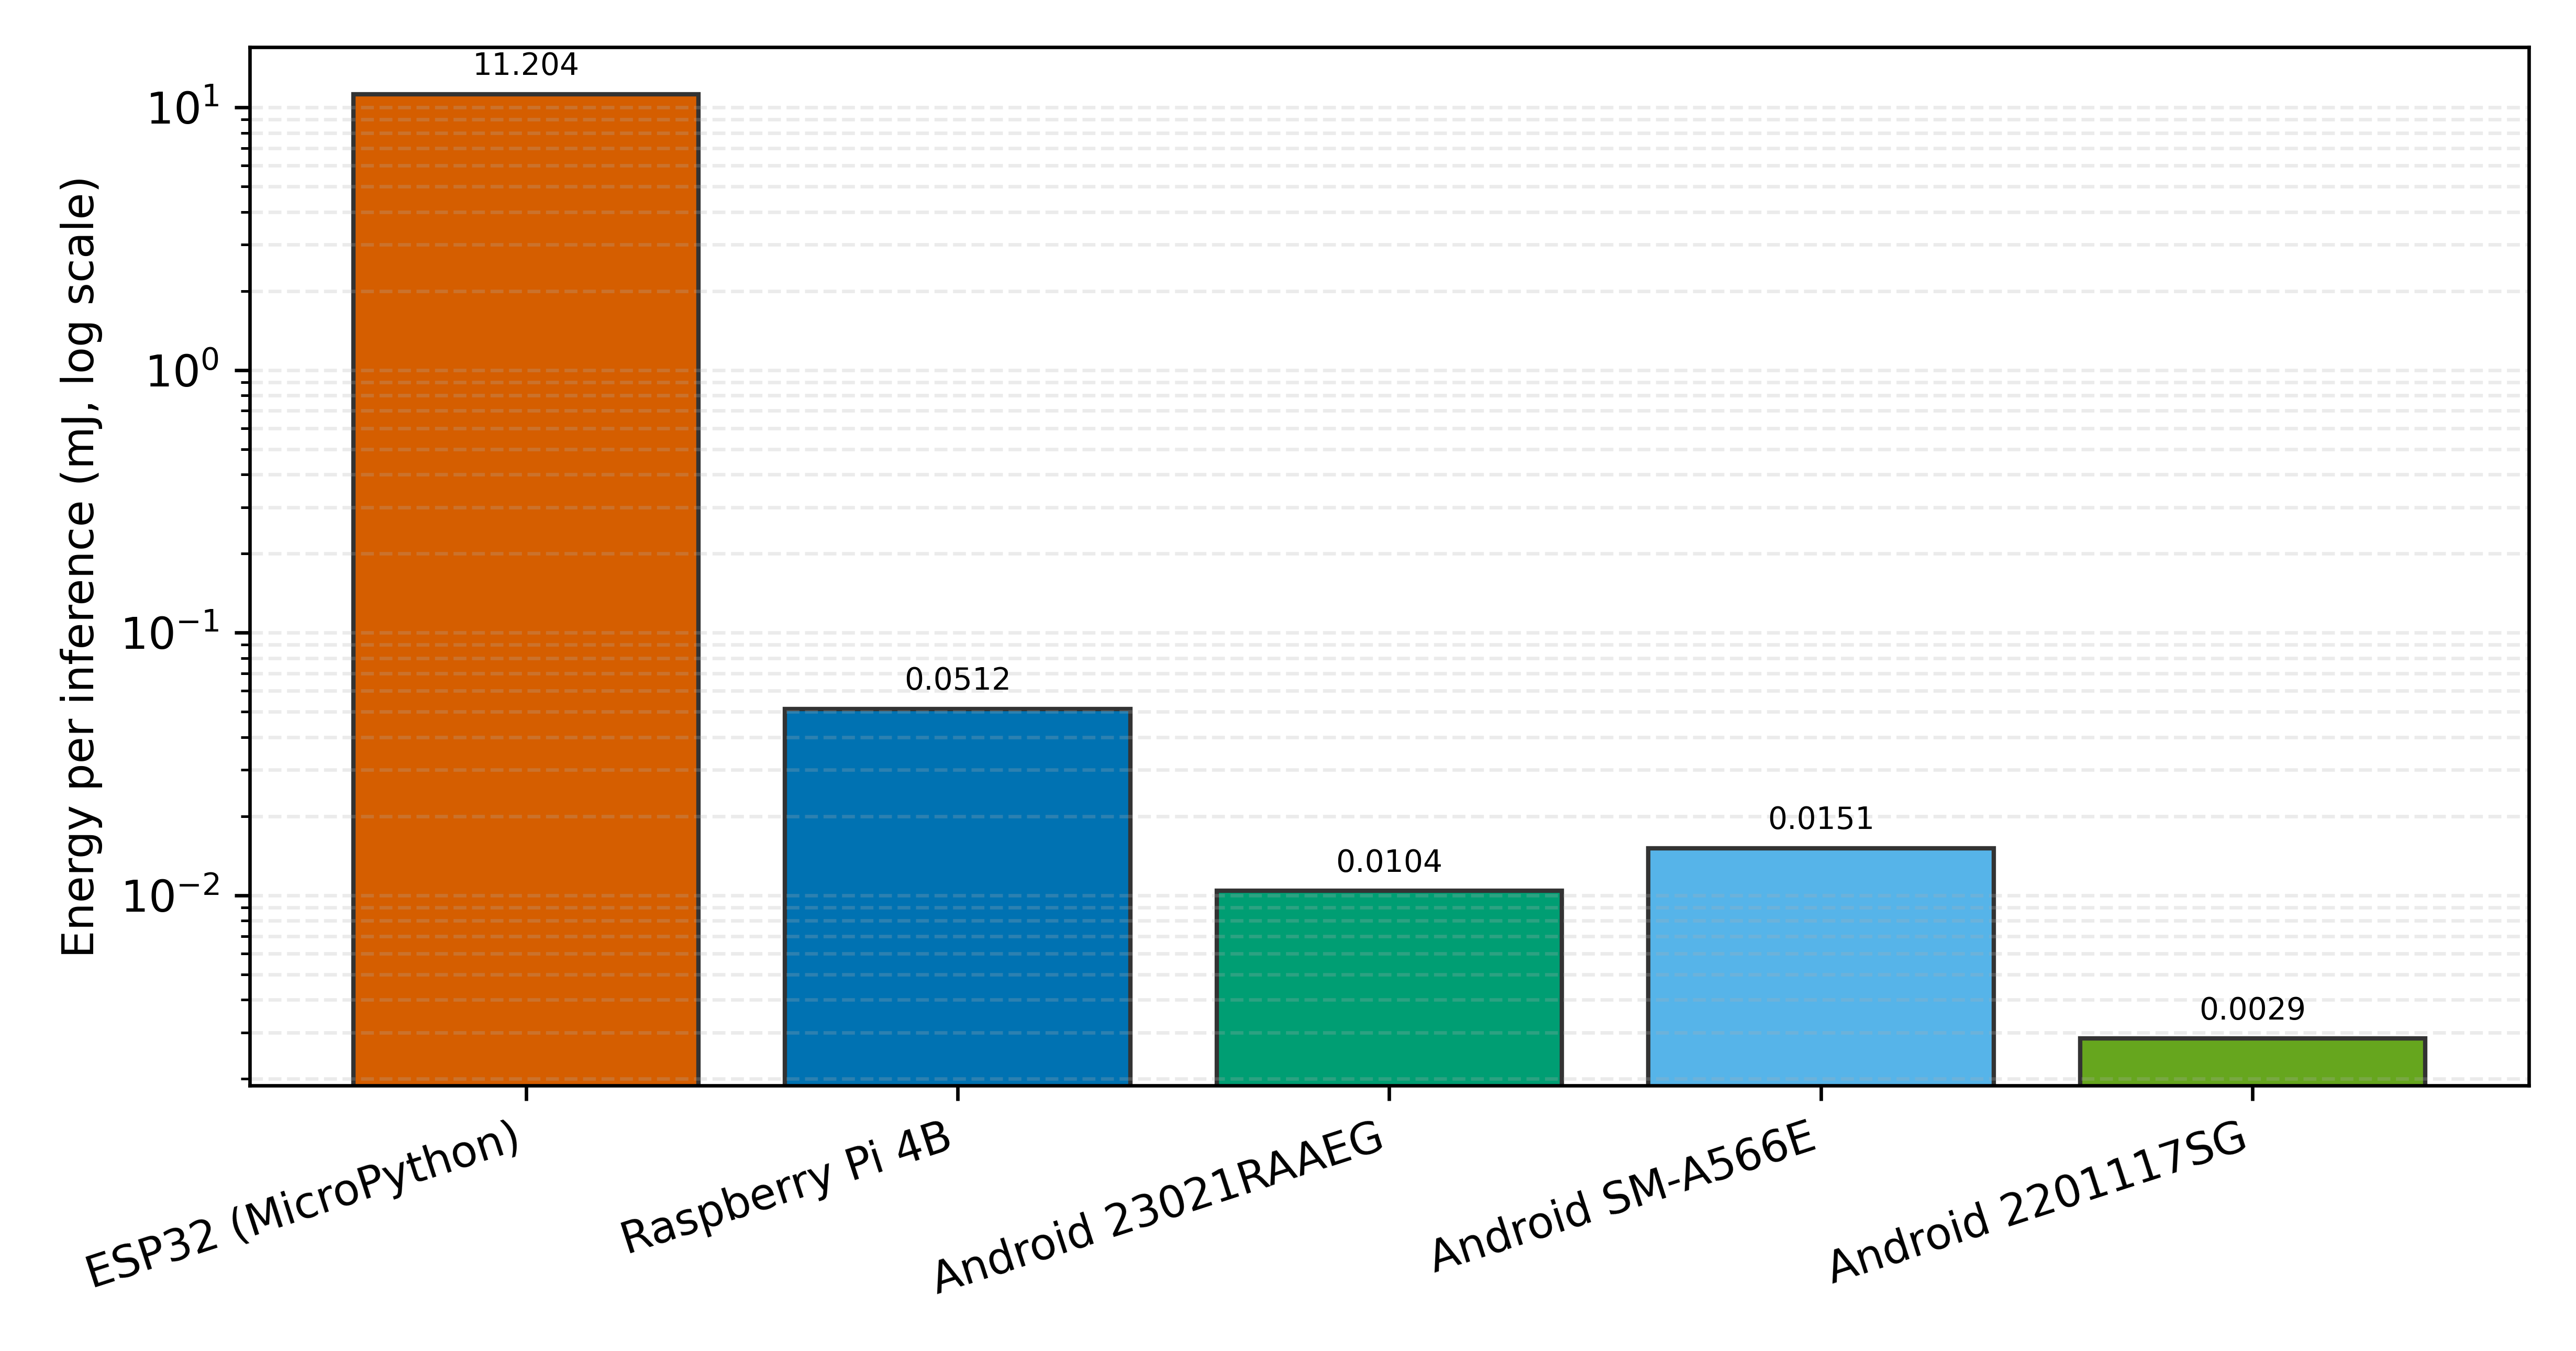
\includegraphics[width=\linewidth]{energy_platforms_bar.png}
\caption{Comparação da energia por inferência (escala logarítmica). \rev{(Figura ampliada nesta revisão para legibilidade dos eixos.)}}
\label{fig:energy_bar_lnncs}
\end{figure}

A Figura~\ref{fig:snn_platform_radar_sba} resume o envelope de implantação multicritério (vazão, latência inversa, energia inversa e referência preditiva) e mostra que nenhuma plataforma domina todos os objetivos: dispositivos Android e Raspberry Pi favorecem amostragem mais densa e fluxos interativos, enquanto o ESP32 permanece relevante para operação esparsa, autônoma e totalmente offline. A figura deve ser lida como um mapa de implantação, e não como um ranqueamento universal.

\begin{figure}[!t]
\centering
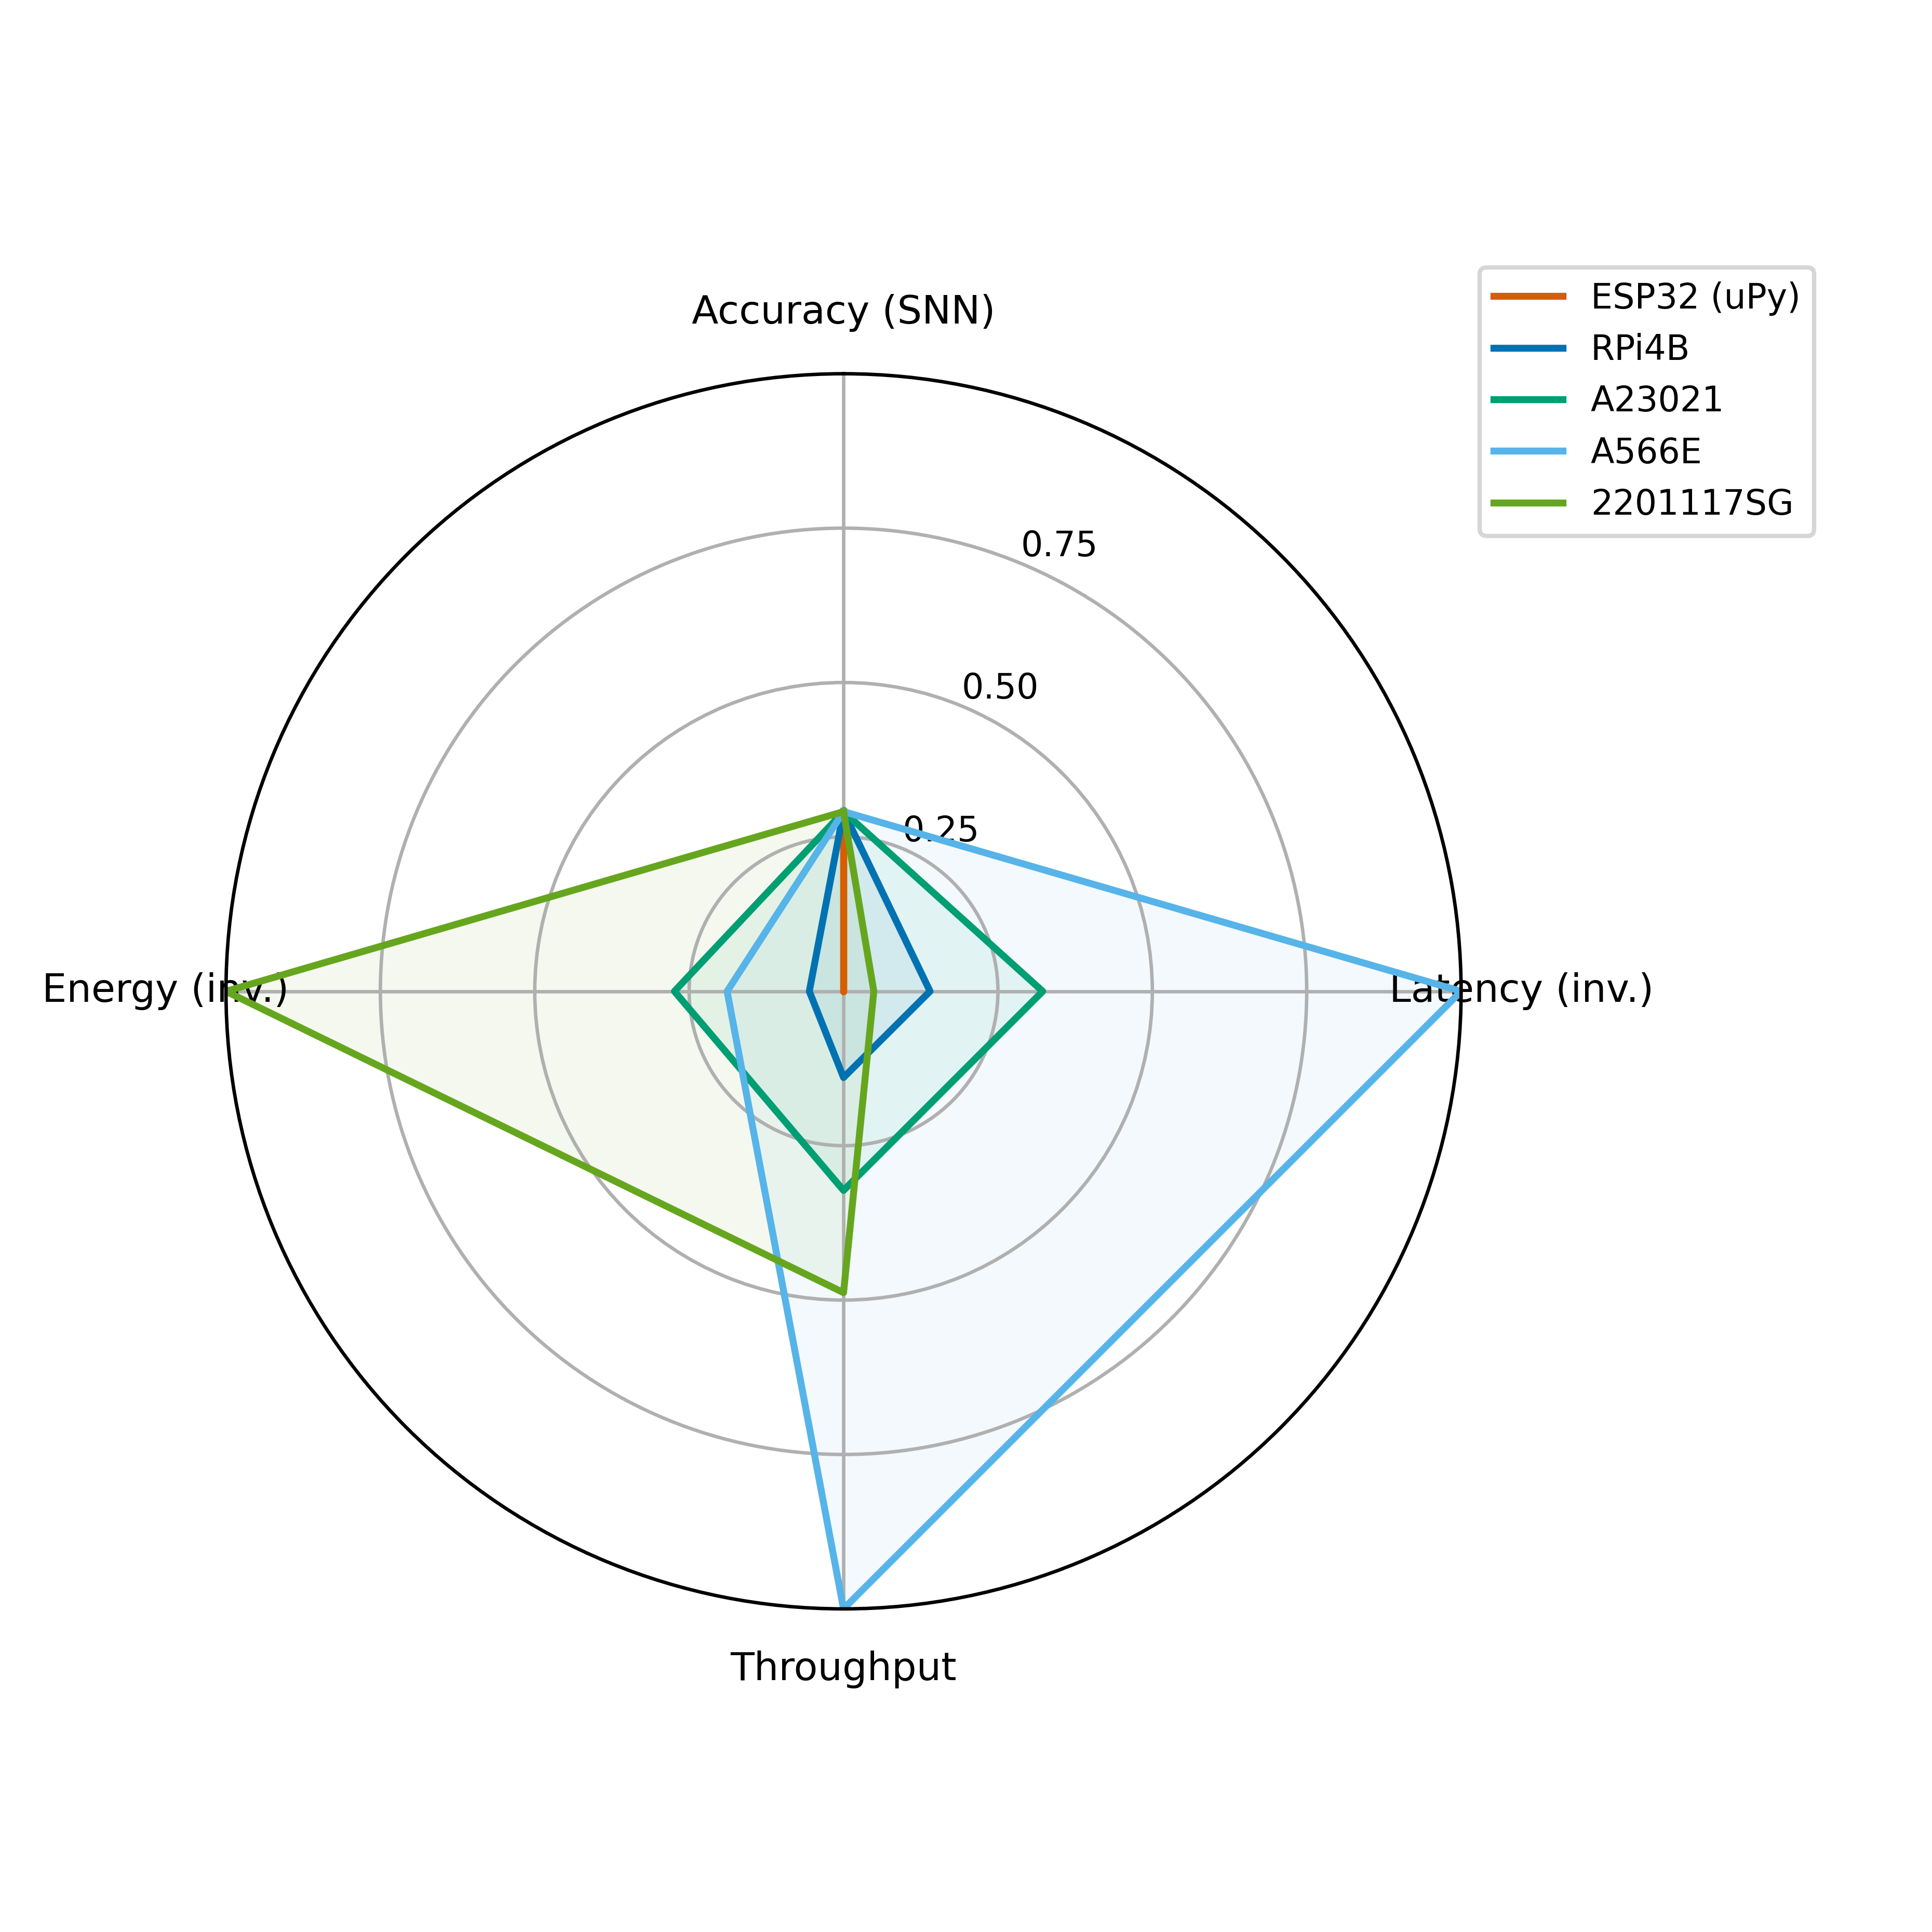
\includegraphics[width=0.52\linewidth]{snn_platform_radar.png}
\caption{Comparação da implantação da SNN entre plataformas usando critérios normalizados (vazão, latência inversa, energia inversa e referência preditiva). \rev{(Figura ampliada nesta revisão para legibilidade dos eixos.)}}
\label{fig:snn_platform_radar_sba}
\end{figure}

\section{Discussão}

Os resultados mostram um claro compromisso entre acurácia preditiva e restrições de implantação. No benchmark com múltiplas sementes, Random Forest e LSTM alcançaram menores erros macro médios, enquanto a SNN permaneceu competitiva e claramente mais estável que o MLP. \rev{Os resultados de Wilcoxon e Friedman, junto com os intervalos de confiança sobrepostos, indicam que Random Forest, LSTM e SNN são estatisticamente indistinguíveis neste conjunto de dados, o que reforça que a SNN deve ser interpretada como uma alternativa robusta orientada à borda, e não como um modelo de melhor acurácia universal.} Do ponto de vista metodológico, a configuração multimodal mostrou-se valiosa porque mantém alvos fisicamente relacionados em um único pipeline de inferência e simplifica a lógica de decisão subsequente em aplicações de campo.

Da perspectiva de sistemas, o comportamento das plataformas é heterogêneo: o Dispositivo B alcançou a maior vazão, o Dispositivo C obteve a menor energia incremental por inferência e o ESP32 forneceu viabilidade offline completa a taxas de processamento muito menores. Como a potência de base das plataformas varia com a arquitetura e o comportamento do sistema operacional, a energia por inferência combinada com a vazão é um critério mais acionável do que watts absolutos isoladamente. A ablação do aumento de dados mostrou melhora modesta mas consistente do MAE macro (2,53\%) e ganho em turbidez, indicando que a expansão sintética controlada ajuda a estabilizar o treinamento neste regime de poucas amostras.

\subsection{Diretrizes Práticas de Implantação}
Os resultados combinados permitem uma diretriz simples de implantação para equipes de campo: para amostragem temporal densa, atualizações frequentes de mapas ou painéis quase em tempo real, a execução em smartphones ou SBCs é preferível; para verificações periódicas esparsas com estrita simplicidade de hardware, o ESP32 permanece viável e operacionalmente atraente, apesar dos maiores valores de mJ/inf.

Um segundo ponto prático é a política de seleção de modelos: em cenários de campo restritos, selecionar apenas pelo MAE mínimo pode ser subótimo. Um critério melhor é um envelope multiobjetivo que combine erro de predição aceitável, comportamento estável entre sementes, vazão da plataforma e energia incremental por inferência, extensível com restrições como orçamento de bateria e cadência de telemetria.

\rev{A escolha da SNN em vez do Random Forest merece justificativa explícita, já que o Random Forest alcançou o menor MAE médio. Primeiro, a diferença de acurácia não é estatisticamente significativa: os testes de Wilcoxon e os intervalos de confiança mostram sobreposição completa entre os dois modelos. Segundo, a SNN oferece propriedades que o Random Forest não possui: computação orientada a eventos cujo custo escala com a atividade de pulsos, um único modelo denso compacto que exporta diretamente para ONNX/TFLite em todas as três classes de plataforma, e compatibilidade futura com aceleradores neuromórficos, nos quais a execução pulsada esparsa pode reduzir a energia bem abaixo das medições em CPU aqui reportadas. Terceiro, o parâmetro de codificação temporal $T$ fornece um controle ajustável de acurácia--energia sem contrapartida em comitês de árvores. A SNN é, portanto, selecionada não como o modelo de menor erro, mas como o modelo estatisticamente equivalente com o melhor envelope de implantação.}

\rev{Quanto a Edge AI versus Cloud AI, o compromisso vai além da computação bruta. A inferência em nuvem oferece modelos maiores e atualizações mais simples, mas em implantações remotas na Amazônia adiciona a energia de rádio, que tipicamente domina o orçamento por amostra, latência e disponibilidade atreladas a enlaces intermitentes, custos recorrentes de conectividade e exposição de dados ambientais brutos a infraestrutura de terceiros. A inferência de borda totalmente offline inverte esse perfil: a energia é limitada pela computação local (aqui medida na escala de $\mu$J a mJ por inferência), o monitoramento continua durante interrupções e apenas resultados agregados precisam de sincronização eventual. Um padrão híbrido --- triagem local com consolidação oportunista em nuvem --- é uma evolução natural do presente pipeline.}

\subsection{Interpretação de Erros e Validade}
Os gráficos de predito vs.\ real indicam um claro perfil de erro dependente do alvo: pH e OD seguem a tendência de identidade com menor dispersão, enquanto a turbidez exibe espalhamento mais amplo. Esse comportamento é coerente com a heterogeneidade de águas doces e reforça que a turbidez deve ser interpretada com margens de confiança mais amplas no uso operacional. Da perspectiva de aplicação, essa assimetria apoia uma estratégia de decisão em camadas: tratar pH e OD como sinais de triagem de curto prazo mais fortes, e usar a turbidez primariamente para sinalizar zonas candidatas a amostragem adicional, e não como gatilho isolado. \rev{Para o oxigênio dissolvido especificamente, a análise por alvo mostra que nenhum modelo avaliado alcança $R^2$ médio positivo, o que aponta para uma limitação do conjunto de atributos, e não da modelagem: as entradas atuais carregam pouca informação relacionada ao OD (\mbox{$|r| \leq 0,24$}). Melhorar a predição de OD exigirá, portanto, enriquecer a modalidade de entrada --- p.~ex., condutividade, potencial de oxirredução, clorofila ou perfis diários de temperatura --- em vez de mais ajuste de modelo.}

As ameaças à validade permanecem centradas no tamanho amostral e na representatividade regional. Embora o aumento de dados, a avaliação com múltiplas sementes e o benchmarking multiplataforma tenham melhorado a robustez, a generalização mais ampla ainda requer campanhas em múltiplas estações e múltiplos sítios, com protocolos de aquisição harmonizados e validação externa repetida. \rev{A transferibilidade para outras regiões deve ser enquadrada em nível de pipeline, e não dos pesos treinados: os gradientes espaciais aprendidos são específicos do Lago do Serpa, de modo que a aplicação direta do modelo ajustado a outro lago não deve preservar a acurácia. O que se transfere é a metodologia --- projeto de atributos, política de aumento, protocolo estatístico e pilha de implantação ---, que pode ser retreinada localmente a partir de uma campanha comparavelmente pequena em um novo sítio. Estratégias de ajuste fino entre sítios e de adaptação de domínio estão planejadas para quantificar explicitamente esse custo de transferência.} A reprodutibilidade é uma força prática deste pipeline: o protocolo de modelagem, a avaliação baseada em sementes e as medições de implantação offline são explícitos e portáveis, permitindo replicação direta em outros contextos de baixa conectividade. Além das métricas preditivas, a implantação no Raspberry Pi alcançou inferência submilissegundo e a validação no ESP32 confirmou execução offline autônoma sob recursos restritos, reforçando que a inferência local é praticável em perfis de borda heterogêneos.

\section{Conclusão}

Este artigo apresentou um pipeline SNN multimodal offline com consciência energética para a predição da qualidade da água em um contexto amazônico de monitoramento na borda. A abordagem proposta demonstrou viabilidade prática do treinamento à implantação, incluindo interpretação geoespacial e benchmarking multiplataforma de latência/energia. Os resultados indicam que a inferência neuromórfica é implantável sob restrições reais de hardware, com compromissos mensuráveis e específicos por plataforma entre vazão e energia por inferência. Embora nem sempre seja a melhor em MAE absoluto, a SNN permanece uma opção robusta quando o processamento temporal orientado a eventos e a compatibilidade com a borda são requisitos de primeira ordem.

As ameaças à validade devem ser explicitamente consideradas na interpretação destes achados. O principal risco à validade interna é o tamanho limitado do conjunto de dados original de campo, que pode aumentar a sensibilidade à partição e tornar pequenas diferenças de métricas instáveis entre partições; isso foi mitigado por avaliação com sementes repetidas, aumento de dados conservador e relato por alvo, mas não totalmente eliminado. A validade externa também é limitada pela diversidade hidrológica entre sub-regiões amazônicas, de modo que afirmações regionais mais amplas requerem campanhas em múltiplos sítios e estações, com protocolos de aquisição harmonizados. Trabalhos futuros incluem aquisição de campo mais ampla ao longo de regimes sazonais, validação externa em sistemas de água doce \rev{e lagos} adicionais, e co-otimização mais profunda dos parâmetros de codificação e dos modos de execução do hardware para melhor equilíbrio energia-desempenho. \rev{As extensões metodológicas planejadas incluem validação cruzada k-fold completa no conjunto de dados ampliado, uma comparação sistemática de estratégias de aumento de dados além da perturbação gaussiana, a medição do consumo de energia de Random Forest, LSTM e MLP sob o mesmo protocolo de repouso/carga usado para a SNN em dispositivos idênticos, e modalidades de entrada enriquecidas para tratar a limitação do oxigênio dissolvido identificada na análise por alvo.} De forma geral, este estudo demonstra que modelos neuromórficos podem apoiar o monitoramento ambiental prático em regiões remotas, viabilizando inteligência de borda com consciência energética para a predição da qualidade da água na Amazônia.

\section*{Agradecimentos}

Os autores agradecem ao Laboratório de Automação, Visão Computacional, Inteligência Artificial e Robótica (NAVIR), ao Programa de Pós-Graduação em Ciência, Tecnologia e Saúde (PPGCTS) e à Universidade Federal do Amazonas (UFAM) pelo apoio institucional.


\bibliography{references_compact}

\end{document}
